\documentclass[a4paper]{article}

\usepackage{listings}
\usepackage[utf8]{inputenc}
\usepackage[T1]{fontenc}
\usepackage[spanish]{babel}
\usepackage[left=2cm, right=2cm, top=2cm, bottom=2cm]{geometry}
\usepackage{setspace}
\usepackage{graphicx}
\usepackage{xcolor}
\usepackage{geometry}
\usepackage{multirow}
\usepackage[hidelinks]{hyperref}
\usepackage{setspace} % Para el espaciado entre lineas
\setstretch{1.2} % Aquí definimos el espaciado en unidades
\usepackage{parskip} %  Para arreglar la forma en la que se manejan los parrafos
\usepackage{fancyhdr}
\usepackage{tikz,lipsum,lmodern}
\usepackage[most]{tcolorbox}
\usetikzlibrary{shapes.geometric, arrows}
\usepackage{appendix}
\usepackage{tocloft} % Paquete para personalizar el índice de figuras
%\usepackage{minted} % Paquete para resaltado de sintaxis
\usepackage{enumitem}
\usepackage{hyperref}
\usepackage{fontawesome5} % Importa el paquete de íconos
\usepackage{pdflscape}

% Sets de dimensiones
\setlength{\parindent}{0pt}
\setlength{\parskip}{0.8em plus 0.5em minus 0.2em}
\setlength{\parfillskip}{\parindent plus 1fill}

% Declaración de variables personalizadas
\newcommand{\logoPortada}{Images/PixelartPisa.png}
\newcommand{\cifplogo}{Images/cifplogo.png}

% Definición de colores
\definecolor{bluePortada}{HTML}{146c8a}

%Adicionales
\setlength{\headheight}{40.2pt}
\pagestyle{fancy}
\fancyhf{}
\lhead{\includegraphics[width=1cm]{\logoPortada}}\rhead{
\includegraphics[width=2cm]{Images/cifplogo.png}}
\renewcommand{\headrulewidth}{3pt}
\renewcommand{\headrule}{\hbox to\headwidth{\color{bluePortada}\leaders\hrule height \headrulewidth\hfill}}

\tikzstyle{startstop}=[rectangle,rounded corners, minimum width=3cm,minimum height= 1cm, text centered,draw=black, fill=red]
\tikzstyle{io}=[trapezium,trapezium left angle=70,trapezium right angle=110,minimum width=3cm,minimum height= 1cm, text centered,draw=black, fill=blue]
\tikzstyle{process}=[rectangle,minimum width=3cm,minimum height= 1cm, text centered,text width= 3cm,draw=black, fill=orange]
\tikzstyle{decision}=[diamond,minimum width=3cm,minimum height= 1cm, text centered,draw=black, fill=green]
\tikzstyle{arrow}=[thick]



\begin{document} % Inicio del documento
\begin{titlepage}
    \centering % para centrar
    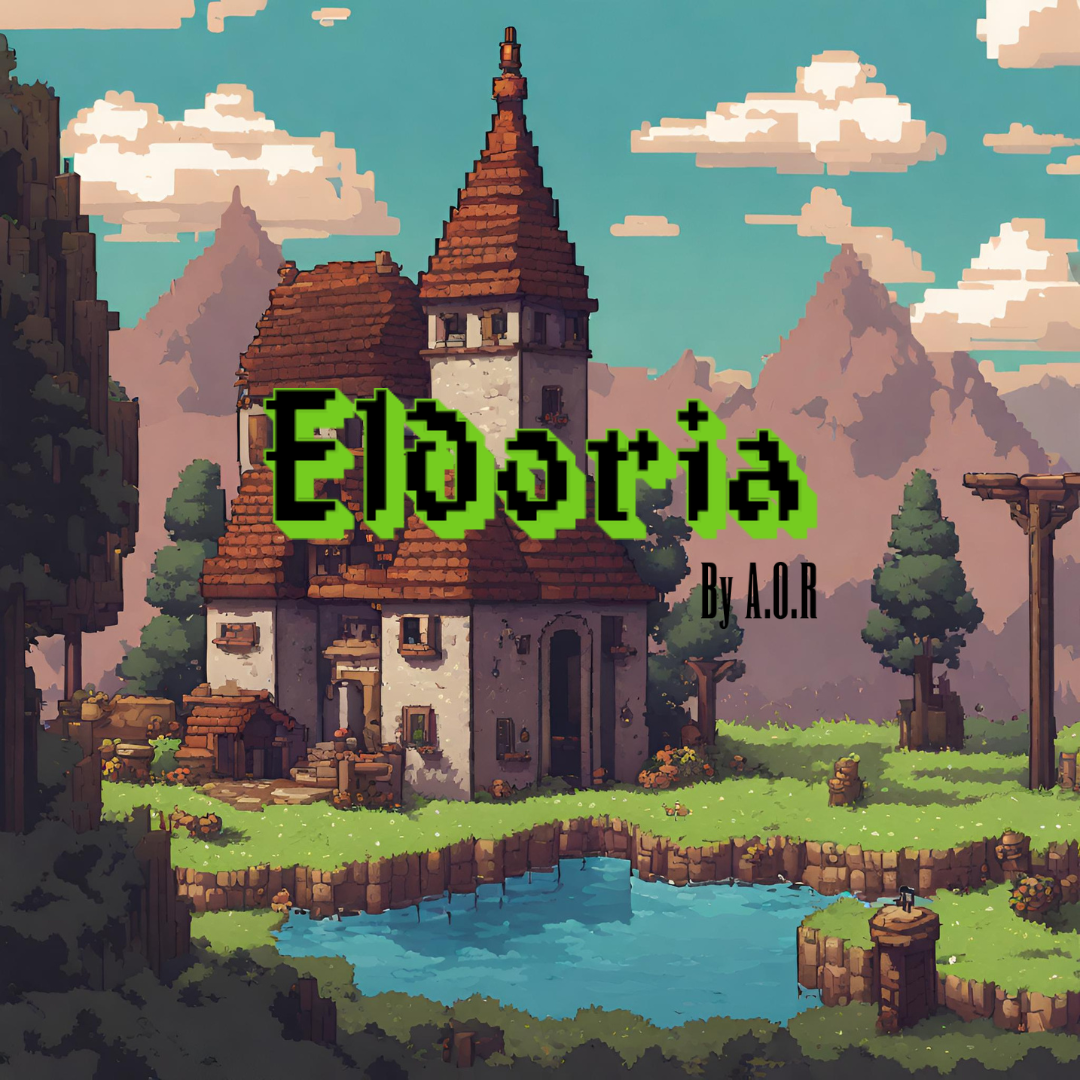
\includegraphics[width=0.5\textwidth]{Images/Eldoria.png}\par
    \vspace{0.4cm}
    {\scshape\LARGE\textbf{Proyecto FP DAM - CIFP LaLaboral}\par} % Contenido de la portada
    \vspace{0.4cm}
    {\LARGE\textcolor{bluePortada}{Eldoria - Alejandro Orviz Recalde}\par}
    \vspace{0.2cm}
    {\Large Tutor y tutora: Alberto Muñóz Blázquez y Marta Elena Menéndez Huerta\par}
\end{titlepage}
% Comienzo del TOC
\clearpage

\tableofcontents
\clearpage

\listoffigures
\clearpage

\listoftables
\clearpage
% ---------------------------------------------------------------------
\section{Agradecimientos}
Este proyecto no sería posible sin la ayuda de varias personas involucradas en este desarrollo. Carles por ayudarme con sus reviews de código,
Laura por darme parte de sus conocimientos en el desarrollo de videojuegos para poder desarrollar bien, Marta la tutora por resolverme dudas y otorgarme
documentación, y por ultimo Miguel por haberme inspirado a realizar este videojuego, el cual está dedicado hacia él.

Las funciones de estas personas me han ayudado en mayor o menor medida a terminar este proyecto de FP, el cual no podría haber acabado sin ayuda, es por ello que reservo
esta parte del docuemnto para agradecer a estas personas su colaboración conmigo, sobre todo a Carles y Laura, los cuales me han apoyado durante todo el desarollo.

\clearpage
% ---------------------------------------------------------------------
\section{Introducción}
El presente proyecto trata sobre un videojuego llamado \textbf{Eldoria}, se encuentra desarrollado en \textit{Java} y es una aventura en 2 dimensiones con gráficos \textit{pixel art}
el cual tendrá una forma de jugar similar a videojuegos antiguos tales como:
\begin{itemize}
    \item The legend of Zelda
    \item The legend of Zelda Minish cap
    \item Final Fantasy I, II, III
    \item Super Mario RPG
\end{itemize}
Algunos datos del proyecto adicionales son:

\begin{table}[ht]
    \centering
    \begin{tabular}{| c | c |}
        \hline
        Título de la aplicación   & Eldoria         \\ \hline
        Autor                     & Alejandro Orviz \\ \hline
        Profesor                  & Alberto         \\ \hline
        Tutora                    & Marta           \\ \hline
        Code reviews              & Carles          \\ \hline
        Desarrollo de videojuegos & Laura           \\ \hline
    \end{tabular}
    \caption{Tabla de participantes}
    \label{tab:participantes}
\end{table}

El videojuego se inspira fuertemente en los primeros juegos creados para la Super Nintendo, por lo que se verán bastantes similitudes tanto en estructura de niveles
como en linealidad e historia del mismo. Además todas las images que se han usado son libres de derechos de autor o en su defecto creadas con inteligencia artificial para evitar problemas de copyright.

\clearpage
% ----------------------------------------------------
\subsection{Motivación}
A día de hoy son muchas las personas que juegan a videojuegos, pero no muchos recuerdan las bases u orígenes de los mismos, en este caso, en mi juego llamado
\textbf{Eldoria} tenemos una aventura en 2 dimensiones en estética \textit{pixel} que nos lleva a un mundo de fantasía el cual nos puede provocar la nostalgia de revivir
videojuegos como \textit{The legend of Zelda 1}. Además este videojuego aprovecha conceptos de programacion sobre lectura, apertura y creación de archivos asi como
conexiones con bases de datos. La duración del mismo aun esta por determinar y depende mas bien de la persona y del tipo de jugador. Con este proyecto se busca
es proveer al usuario, de un tiempo de ocio en el que pueda disfrutar pasando el tiempo frente a retos y acertijos propuestos por el videojuego.

\subsection{Inspiraciones}
Este juego además tiene varias inspiraciones en el mundo moderno y \textit{retro}, pasaremos a explicar en profundidad sus inspiraciones, las cuales incluyen tambien documentos realizados por otra gente como veremos a contiuación:\\
\begin{enumerate}
    \item \textbf{The legend of Zelda}
          \begin{itemize}
              \item \textit{The legend of Zelda} es un videojuego japonés de los años 80, el cual fue desarrollado por Nintendo. Se trata de un videojuego de aventuras, puzzles y acción, fue un referente en su época y a día de hoy se considera la base de los juegos de aventuras.
              \item El objetivo dentro del juego es simple, nuestro protagonista \textit{Link}, debe rescatar a la princesa \textit{Zelda} de las garras del \textit{Rey Demonio}, para ello tendrá que recorrer \textit{Hyrule} en busca de objetos, armas, conocimiento, etc \dots
              \item Hablando de temas tecnicos, el juego se considera un \textit{RPG (Role playing game)}, es decir, un juego de rol, de perspectiva aérea que cuenta con varios puzzles para superar algún nivel. En tema de gráficos, encontramos una estética \textit{pixel art} la cual, no requiere un desarrollo super extenso.
              \item Aunque a día de hoy existen varios videojuegos de \textit{The legend of Zelda}, nosotros nos fijaremos en el primero ya que es el que dejó las bases para el resto de los juegos de la saga, es por eso que el videojuego, en estética y jugabilidad, bebe mucho de esta obra.
          \end{itemize}
    \item \textbf{Final fantasy}
          \begin{itemize}
              \item \textit{Final fantasy} es un videojuego de rol japonés desarrollado por \textit{Square.Co(Más tarde conocida como "Square Enix")}, el cual fue un gran pilar en la industria de los videojuegos de rol de la época y actuales, salió en el año 1987, y fue el inicio de una saga de videojuegos que a día de hoy continua su desarrollo(\textit{Actualmente existe el "Final Fantasy XVI"})
              \item La historia de este juego, trata acerca de 4 personajes que van en busca de unos cristales mágicos para vencer el mal que acecha el mundo, esta historia se repetirá en mayor o menor medidad en los próximos juegos de la saga. Su estética es similar al juego previo hablado, \textit{The legend of Zelda}, pues ambos juegos salieron casi en el mismo año y en una época donde el hardware, no era tan potente como ahora.
          \end{itemize}
    \item \textbf{TFG de la Escuela de ingenieria de Segovia}
          \begin{itemize}
              \item Para este proyecto primero, hemos investigado las opciones ya creadas por la gente, en caso de que existieran, en este caso hemos encontrado un TFG (\textit{Estará adjuntado en la parte de Bibliografia}), el cual nos habla acerca del desarrollo de un videojuego móvil con unity, este TFG, nos ha servido de ayuda ya que nos ha provisto de una estructura de desarrollo, enlaces de interés e ideas para el desarrollo.
          \end{itemize}
\end{enumerate}

\subsection{Herramientas usadas}
En esta sección, explicaremos brevemente las herramientas usadas, y el por qué de las mismas, así como su coste en el caso de que sean de pago.

Para el desarrollo de este proyecto de FP, se han usado las siguientes herramientas:
\begin{enumerate}
    \item \textbf{IntelliJ Idea Community y Ultimate}
          \begin{itemize}
              \item \textit{IntelliJ} es nuestro IDE de preferencia, el cual nos provee de varias herramientas útiles y necesarias para el desarrollo del proyecto, se trata de un entorno de desarrollo, lanzado en 2001, el cual cuenta con dos versiones, una gratuita y otra de pago, en este proyecto usaremos principalmente la gratuita, aunque necesitaremos una funcionalidad de la versión de pago.
              \item Este entorno de desarrollo cuenta con una tecnología de sugerencias de código real, bastante avanzada la cual nos provee de código por lo general bastante acertado según lo que estamos desarrollando, ya que mientras programamos, el IDE, analiza lo que estamos escribiendo y lo que hemos programado para darnos mejores sugerencias de autocompletado.
              \item \textbf{El precio de este IDE, actualmente(Mayo/2024) es de: 160 euros al mes}
          \end{itemize}
          \begin{figure}[!ht]
              \centering
              
\includegraphics[width=0.1\textwidth]{Images/IntelliJ_IDEA_Icon.svg.png}
              \caption{Logo de IntelliJ IDEA}
              \label{fig:intellij}
          \end{figure}

    \item \textbf{XAMPP}
          \begin{itemize}
              \item \textbf{XAMPP} es un paquete de software gratuito y de código abierto desarrollado por Apache Friends, que proporciona una solución fácil de instalar para configurar un servidor web local. XAMPP incluye Apache, MySQL (o MariaDB), PHP y Perl, entre otros componentes.
              \item El nombre \textit{XAMPP} es un acrónimo que viene de:
                    \begin{itemize}
                        \item X: Plataforma cruzada (Cross-platform)
                        \item A: Apache (servidor web)
                        \item M: MySQL o MariaDB (sistema de gestión de bases de datos)
                        \item P: PHP (lenguaje de scripting del lado del servidor)
                        \item P: Perl (lenguaje de programación)
                    \end{itemize}
          \end{itemize}
    \item \textbf{JDBC}
          \begin{itemize}
              \item \textbf{JDBC} tambien conocido como \textit{Java Database Connectivity}, es la especificación JavaSoft de una interfaz de programación de aplicaciones (API) estándar que permite que los programas Java accedan a sistemas de gestión de bases de datos. La API JDBC consiste en un conjunto de interfaces y clases escribas en el lenguaje de programación Java
              \item Hemos usado esta biblioteca debido a su facilidad de uso, que nos permite hacer consultas de una manera muy cómoda.
              \item Además proporciona un marco estándar para la conexión, consulta y manipulación de datos, asegurando la portabilidad y flexibilidad de las aplicaciones Java.
          \end{itemize}
    \item \textbf{Visual studio Code}
          \begin{itemize}
              \item \textbf{Visual studio Code} es un IDE, que nos provee de una cantidad de configuraciones infinita, y también al tener esta versatilidad es perfecto como IDE, para trabajar en un proyecto que involucre usar varios lenguajes a la vez, aunque en nuestro caso, lo hemos usado para desarrollar el documento \LaTeX, de la memoria del proyecto.
              \item Para desarrollar el documento, hemos tenido que descargarnos \textit{Perl}, \textit{LaTeX Workshop} y por ultimo \textit{MikTex}, esto es necesario si queremos que Visual Studio nos deje desarrollar cualquier docuemnto \LaTeX, además de un plugin para poder visualizar el documento pdf compilado desde Visual Studio.
          \end{itemize}
          \begin{figure}[!ht]
              \centering
              
\includegraphics[width=0.2\textwidth]{Images/Visual_Studio_Code_1.18_icon.png}
              \caption{Logo de Visual studio code}
              \label{fig:visualstudio}
          \end{figure}
    \item \textbf{\LaTeX}
          \begin{itemize}
              \item \textbf{\LaTeX} es un sistema de composición de textos orientado a la creación de documentos escritos que presenten una alta calidad tipográfica. Por sus características y posibilidades, se usa de forma especialmente intensa en la generación de artículos y libros científicos que incluyen, entre otros elementos, expresiones matemáticas.
              \item \textbf{\LaTeX} está formado por un gran conjunto de macros de \textbf{TeX}, escrito por Leslie Lamport en 1984 con la intención de facilitar el uso del lenguaje de composición tipográfica \LaTeX, creado por Donald Knuth. Se utiliza mucho para la composición de artículos académicos, tesis y libros técnicos, dado que la calidad tipográfica de los documentos realizados en LaTeX se considera adecuada a las necesidades de una editorial científica de primera línea, muchas de las cuales ya lo emplean.
              \item Para poder desarrollar el documento de la memoria en \LaTeX, hemos hecho uso de la documentación que existe en internet, asi como documentos ya hechos, por ejemplo repositorios de gente que ya ha realizado un documento \LaTeX, aunque la plantilla usada en este documento esta realizada desde cero.
          \end{itemize}
          \begin{figure}[!ht]
              \centering
              
\includegraphics[width=0.2\textwidth]{Images/LaTeX_project_logo_bird.svg.png}
              \caption{Logo de LaTex Project}
              \label{fig:latexlogo}
          \end{figure}
    \item \textbf{MySql}
          \begin{itemize}
              \item \textbf{MySql} es un sistema de gestión de bases de datos relacional desarrollado bajo licencia dual: Licencia pública general/Licencia comercial por \textit{Oracle Corporation} y está considerada como la base de datos de código abierto más popular del mundo, y una de las más populares en general junto a \textit{Oracle} y \textit{Microsoft SQL Server}, todo para entornos de desarrollo web.
              \item \textbf{MySql} fue inicialmente desarrollado por \textit{MySQL AB} (empresa fundada por David Axmark, Allan Larsson y Michael Widenius). \textit{MySQL AB} fue adquirida por \textit{Sun Microsystems} en 2008, y ésta a su vez fue comprada por \textit{Oracle Corporation} en 2010, la cual ya era dueña desde 2005 de Innobase Oy, empresa finlandesa desarrolladora del motor \textit{InnoDB} para \textit{MySQL}. Fácil de usar y simple de implementar. Razones por las cuales, es tambien una de las más usadas.
          \end{itemize}
          \begin{figure}[!ht]
              \centering
              
\includegraphics[width=0.25\textwidth]{Images/MySQL-Logo.png}
              \caption{Logo de MySQL}
              \label{fig:MYSQLLOGO}
          \end{figure}
    \item \textbf{JDK 21}
          \begin{itemize}
              \item \textbf{JDK o \textit{Java Development Kit}} es una serie de herramientas de desarrollo que nos permite crear software en \textit{Java}, además de poder ejecutar archivos \textit{"Jar"} desarrollados con esta \textit{JDK}. Hemos decidido usar la última versión para estar libres de problemas de que nos hagan falta paquetes o de vulnerabilidades.
          \end{itemize}
    \item \textbf{Github Repositories}
          \begin{itemize}
              \item Para poder tener un sistema de control de versiones hemos optado por usar los repositorios de \textit{Github}, los cuales de forma gratuita nos dejan tener un sistema de control de versiones que nos permite mantener de forma sincronizada en varios equipos el mismo proyecto, en nuestro caso el repositorio es público, en caso de quererlo privado, tendríamos o bien que pagar o bien disponer de un servidor local con el que poder tener subido el repositorio en él mediante \textit{Git}.
          \end{itemize}
    \item \textbf{Excalidraw}
          \begin{itemize}
              \item \textbf{Excalidraw} es una web que nos ofrece una pizarra virtual en la que poder dibujar, hacer notas o generar diagramas incluso, como los diagramas UML de software, además cuenta con bastantes opciones a la hora de exportar lo dibujado, y es una herramienta muy útil para hacer esquemas.
          \end{itemize}
          \begin{figure}[!ht]
              \centering
              
\includegraphics[width=0.2\textwidth]{Images/logoExcalidraw.png}
              \caption{Logo de Excalidraw}
              \label{fig:excalidraw}
          \end{figure}
\end{enumerate}
\clearpage
%-----------------------------------------------------
\subsection{Primeras metas}
\begin{enumerate}
    \item \textbf{Realizar un personaje que se mueva en pantalla}
          \begin{itemize}
              \item El principal punto sobre el que podemos avanzar es mostrar el personaje en pantalla y ser capaces de moverlo con las teclas del teclado, que el programa sea capaz de saber si queremos ir a las 4 direcciones posibles y que se mueva con cierta fluidez.
          \end{itemize}

    \item \textbf{60 Frames por segundo}
          \begin{itemize}
              \item Una de las metas tambien principales es limitar el rendimiento del juego ya que queremos que se dibuje lo que hay en pantalla 60 veces por segundo, si no ponemos un limitador, esta cifra sería mucho más alta, lo que nos podria provocar problemas, llegados a un número muy alto de interacciones.
          \end{itemize}

    \item \textbf{Colisiones}
          \begin{itemize}
              \item Dentro de un videojuego queremos que se produzcan colisiones con el personaje o personajes del juego, no queremos que se atraviesen muros, o cosas de ese estilo, por lo que esta es una de las principales metas a superar.
          \end{itemize}

    \item \textbf{Menús de juego}
          \begin{itemize}
              \item También queremos realizar pantallas de estado del personaje, menú principal, diálogos, menú de pausa, etc \dots
          \end{itemize}

    \item \textbf{Sistema de combate}
          \begin{itemize}
              \item Al ser un juego de rol y aventuras, queremos incluir algún enemigo y algun sistema de combate en el que se pueda dar y recibir daño asi como barras de vida para los enemigos, o para el jugador.
          \end{itemize}

    \item \textbf{Pantalla Completa}
          \begin{itemize}
              \item Otra meta sería poder ejecutar el juego en pantalla completa sin bordes, es un pequeño punto de estética.
          \end{itemize}

    \item \textbf{Interfaces}
          \begin{itemize}
              \item Una de las metas es obviamente realizar menús y aprovechar los primeros conocimientos de \textit{Diseño y desarrollo de Interfaces} para poder realizar ventanas dentro del juego.
          \end{itemize}

    \item \textbf{Empaquetar el juego}
          \begin{itemize}
              \item La última meta propuesta es empaquetar el juego y poder tener algún ejecutable para poder llevarlo a \textit{"todas partes"}.
          \end{itemize}
\end{enumerate}

\clearpage
% --------------------------------------------
\section{Planificacion y presupuesto}
\subsection{Planificacion}
Este proyecto se ha desarrollado en varias fases como un desarrollo real en un entorno empresarial, empezando en \textit{Octubre de 2023}(los totales de horas son aproximados).
\subsection{Septiembre - 2023}
En esta fase comenzó el descarte de ideas y la lluvia de las misma para saber más o menos que podríamos hacer en cuanto a proyecto se refiere.
\begin{flushright}
    \bf Total de horas: 10 horas
\end{flushright}

\subsection{Octubre - 2023}
En la primera fase del mismo se ha pensado la idea y hecho una planificación inicial del mismo, así como varios apuntes sobre la tecnología a usar, la cual ha recibido cambios en el desarrollo.
\begin{flushright}
    \bf Total de horas: 20 horas
\end{flushright}

\subsection{Noviembre - 2023}
En esta fase empezamos los primeros pasos del desarrollo y encontramos las primeras dificultades del mismo, como por ejemplo:
\begin{itemize}
    \item Assets
    \item Falta de conocimiento
    \item Desconocimiento de la BDD
    \item Diseño de la BDD
\end{itemize}
Teniendo estas dificultades claras continuamos un desarrollo temprano de una pequeña version bastante primitiva del proyecto que nos servirá de base para poder continuar con él. En esta versión declaramos las bases del programa final que tendremos por el final del proyecto.
\begin{flushright}
    \bf Total de horas: 30 horas
\end{flushright}

\clearpage
\subsection{Diciembre - 2023}
En esta fase continuamos un poco más el desarrollo y adelantamos un poco del mismo de cara a la siguiente fase, ya que en el momento que hemos acabado la fase de primeros pasos el resto que se realice antes del anteproyecto es trabajo adelantado, dentro de esta fase el principal problema que nos hemos encontrado ha sido \textbf{el tamaño del heap de Java}, siendo este el principal limitante a la hora de realizar un diseño de niveles grande como se tenía pensado principalmente. Este problema nos produjo un cambio de planes ya que el mapa que inicialmente se habia pensado en un mapa de 100x100 casillas se tuvo que reducir a 50x50, es decir la mitad, esto nos deja para las pruebas del desarrollo un mapa de 25x25 que más tarde será de 50x50. Este cambio viene de la famosa excepcion \textit{"java.lang.OutOfMemoryError: Java heap space"}.\\
Este problema se produce al dibujar el mapa del videojuego, ya que el heap no es capaz de almacenarlo y entonces nos devuelve esa excepción, para corregirlo, lo que hemos hecho ha sido disminuir el tamaño del mapa a uno más pequeño, si bien es cierto que se puede aumentar la memoria del heap de java mediante comandos, hemos preferido dejarlo como está y disminuir el mapa.\\
Otros datos interesantes de esta fase han sido los progresos en el desarrollo y la nueva replanificación del mismo, ya que al tener el error del heap de java, hemos tenido que reestructurar partes del desarrollo ya planificadas.
\begin{flushright}
    \bf Total de horas: 50 horas
\end{flushright}

\subsection{Enero/Febrero/Marzo - 2024}
Dentro de esta fase tendriamos la parte referente al anteproyecto. El desarrollo del documento del anteproyecto se realizó usando \LaTeX, y \textit{Overleaf (Una pagina dedicada a escribir documentos LaTeX de forma online)}. La plantilla usada en ese documento es una plantilla creada desde cero con los conocimientos de ese momento acerca del lenguaje, y tambien cogiendo cosas de documentación, foros y proyectos ya hechos de otra gente, es el caso de foros como \textit{StackExchange} en su parte referente al lenguaje, repositorios de github con determinadas funciones que he necesitado poner en el documento, etc\dots \\
Por último dentro del anteproyecto se han escrito cosas acerca de funcionalidad finales que no se han podido cumplir por falta de tiempo, estos comentarios se tendrán en cuenta como \textit{propuestas de mejora}, las cuales son pequeñas o grandes funcionalidades que pueden mejorar o hacer más divertido el juego.
\begin{flushright}
    \bf Total de horas: 40 horas
\end{flushright}

\clearpage
\subsection{Abril/Mayo - 2024}
La penultima fase del proyecto, en esta se encontraria la recta final de desarrollo en la que ya nos ponemos en serio con el mismo y ultimamos los detalles del programa, ademas de añadir todo lo que podamos hasta el dia 3 de junio, el cual es la fecha limite que hemos planificado como \textit{deadline}. Durante esta fase hemos tenido ayuda, bien sea de docuemntación, foros, videos o incluso personas, en esta fase hemos recibido en concreto ayuda de 3 personas, la primera sería la tutora encargada del mismo, que nos ha proporcionado, docuemntación y links de interés para resolver las dudas surgidas, la segunda en este caso sería Laura, una desarrolladora de videojuegos que nos ha dotado de consejos a lo largo del desarrollo y pautas que hemos podido seguir asi como webs donde buscar assets gratis, y por ultimo, Carles, que se trata de un desarollador titulado en DAM, el cual se ha encargado de hacer \textit{code reviews} sobre el codigo del proyecto y el cual nos ha dicho pequeños aspectos que se nos han pasado a la hora de desarrollar, como los comentarios o la indentación correcta.
\begin{flushright}
    \bf Total de horas: 120 horas
\end{flushright}

\subsection{Junio - 2024}
Última fase del proyecto en la que nos hemos centrado en la documentación del mismo aunque se ha hecho de manera transversal, pero se han dado los últimos retoques en esta fase ya que el desarrollo acabó el día 3. Dentro de esta fase hemos buscado muchas funciones y curiosidades para poder hacer un documento parecido a un TFG universitario pero a menor escala, para ello hemos visualizado y leído varios TFGs, de varias universidades de España y hemos tenido la suerte de poder tenerlos descargados para poder ver la estructura de los mismos, como se han escrito y tambien como se han desarollado las personas que los han realizado. Además se ha investigado sobre cómo realizar ciertas cosas dentro de la documentación, como varios índices, imágenes en un formato determinado, etc \dots
\begin{flushright}
    \bf Total de horas: 70 horas
\end{flushright}

\subsection{Diario de horas del proyecto}
\begin{table}[ht]
    \centering
    \begin{tabular}{|c|c|c|c|}
        \hline
        \textbf{Tarea}                                             & \textbf{Fecha de Inicio} & \textbf{Fecha de Fin} & \textbf{Horas Planificadas} \\
        \hline
        Diseño de Juego                                            & 20/08/2023               & 07/02/2024            & 20                          \\
        \hline
        Desarrollo del juego                                       & 08/01/2024               & 03/06/2024            & 220                         \\
        \hline
        Pruebas y Depuración                                       & 03/06/2024               & 10/06/2024            & 30                          \\
        \hline
        Diseño de Niveles                                          & 10/01/2024               & 10/01/2024            & 15                          \\
        \hline
        Apartado artístico de personajes                           & 04/10/2024               & 10/04/2024            & 25                          \\
        \hline
        Documentación                                              & 10/09/2023               & 10/06/2024            & 70                          \\
        \hline
        \multicolumn{3}{|r|}{\textbf{Total de Horas Planificadas}} & \textbf{380}                                                                   \\
        \hline
    \end{tabular}
    \caption{Tabla de horas}
    \label{tab:planificacion-horas}
\end{table}
\clearpage
% -----------------------------------------
\subsection{Presupuesto}

Dentro de esta parte del proyecto hemos intentado abaratar en algunas partes costes y en otras no nos ha quedado más remedio que tener que pagar, ya que o bien nos ofrecen un servicio/funcionalidad que necesitamos o bien es un programa con el que estamos muy familiarizados. Por lo que en este apartado explicaremos parte de las herramientas usadas, ya que algunas son de pago. \\
\subsubsection{IntelliJ Idea}
Empezamos esta sección con nuestro IDE de preferencia, el cual nos provee de bastantes funcionalidades en su versión community, pero en este caso hemos hecho uso de la versión Ultimate, ya que nos realiza el diagrama de clases el mismo IDE, aunque tenemos la licencia educativa, la cual nos deja tener este producto durante nuestros estudios de forma gratuita, hemos optado por incluirlo en el presupuesto ya que sigue siendo una herramienta de pago. \\
\begin{flushright}
    \bf Su precio es de: 160 euros al año
\end{flushright}

\subsubsection{Horas de trabajo}
Teniendo en cuenta la media ofrecida por \textit{Glassdor} acerca de lo que puede cobrar un desarrollador de software Java, hemos visto que su sueldo debería ser cercano a 2000 euros, este sueldo si tenemos en cuenta los meses de desarrollo y horas nos sale lo siguiente.\\
Haciendo cálculos, poniendo como sueldo 1830 euros mensuales y viendo las horas del proyecto y el tiempo, deberiamos cobrar \textbf{25620 euros netos}. Esta cifra sería si estuvieramos en una empresa la cual nos cobra por mes, pero al presentar el supuesto de ser un autonomo, deberiamos cobrar \textbf{1960 euros netos} si tenemos en cuenta las horas totales del proyecto, por lo que tomaremos esta cifra mejor.
\begin{flushright}
    \bf Coste de horas: 10.78 euros la hora
\end{flushright}

\subsubsection{Equipo usado}
El equipo usado para el desarrollo ha sido un ordenador portatil HP, con un intel core i7 de undecima generación, 16gb de RAM, y un ssd de 512GB, el precio del equipo sin ninguna oferta sería de 820 euros.
\begin{flushright}
    \bf Coste del equipo de desarrollo: 820 euros
\end{flushright}
\subsubsection{Tabla de presupuesto}
\begin{table}[ht]
    \centering
    \begin{tabular}{|c|c|}
        \hline
        \textbf{Sección}               & \textbf{Coste}     \\
        \hline
        IntelliJ                       & 160 €              \\
        \hline
        Horas de trabajo               & 10.78 €/hora       \\
        \hline
        Equipo usado                   & 820 €              \\
        \hline
        Equipo usado en pruebas        & 1350 €             \\
        \hline
        \textbf{Total del presupuesto} & \textbf{6.426,4 €} \\
        \hline
    \end{tabular}
    \caption{Tabla del presupuesto}
    \label{tab:presupuesto-table}
\end{table}


\clearpage
% --------------------------------------------
\section{Estudio de mercado y viabilidad de la propuesta}
\subsection{Aplicaciones ya existentes}
Este tipo de videojuego ya existe, siendo claros ejemplos, \textbf{Final Fantasy 1}, \textbf{The legend of Zelda} o incluso \textbf{Pokémon rojo}, este tipo de
programas que han sido desarrollados hace años, tienen en común que siguen la estética \textit{pixel art} y en ellos se entiende, ya que por circunstancias temporales,
no existía nada mejor. En este caso son ejemplos válidos \textit{Sea of stars} el cual fue lanzado en el año 2023, siguiendo también una estética \textit{retro}, y también siguiendo
un género parecido a los juegos ya mencionados.
\subsection{Viabilidad}
Dentro de este proyecto nos enfrentamos a varios obstáculos y decisiones que nos van a hacer tardar más o tardar menos en desarrollar el proyecto.
Los principales obstáculos que nos hemos encontrado han sido:
\begin{itemize}
    \item \textbf{Desconocimiento de la lógica de un videojuego:} \\
          La principal dificultad de este punto ha sido la poca familiaridad de la creación de un programa que funcione como un videojuego, ya que se requiere una lógica distinta a la que estoy familiarizado.

    \item \textbf{Desconocimiento en LaTeX:} \\
          A pesar de haber escogido LaTex para realizar el documento, el principal obstáculo ha sido tener en cuenta casi todos los aspectos de formato bonito para el documento, ya que la falta de experiencia
          documentando en LaTeX ha hecho complicado poder seguir de forma fluida el proyecto

    \item \textbf{Desconocimiento en la gestión de memoria:} \\
          La gestión de memoria es crucial en el desarrollo de software. La falta de entendimiento de este aspecto nos ha provocado un problema de rendimiento en las etapas tempranas del desarrollo.

    \item \textbf{Diseño de niveles:} \\
          En el caso de este punto ya que carecemos de teoría acerca de niveles se ha hecho complicado poder realizar un mapa competente ya que carece de una tecnicidad o complejidad excesiva.

    \item \textbf{Diseño de personajes:} \\
          En cuanto a los personajes se ha optado por usar galerias gratuitas, el principal obstáculo ha sido cuadrar los sprites ya que cada uno viene de autores diferentes y no puede quedar todo diferente.

    \item \textbf{Implementación de base de datos:} \\
          El principal problema de la implementación de la base de datos, ha sido el qué guardamos en la base de datos, ya que no podemos guardar algo que se tenga que consultar cada poco, por que provocaría
          en este caso problemas de rendimiento.

    \item \textbf{Desconocimiento de herramientas:} \\
          Uno de los principales problemas y lastres, a la hora del desarrollo es el hecho de no contar con las suficientes herramientas, ya sea para diseñar niveles, personajes, o automatizar procesos

    \item \textbf{Desarrollo parcialmente solitario:} \\
          Si bien es cierto que contamos con ayuda de la tutora correspondiente para realizar el TFG, no contamos con un desarrollador al lado que pueda ver quizás optimizaciones o refactorizaciones que nosotros no.

    \item \textbf{Envergadura del proyecto:}\\
          En fases finales del proyecto, el tiempo ha sido un factor importante, el cual ha podido incluso decidir por nosotros que funciones metemos y cuales no.
\end{itemize}


\clearpage
% -------------------------------------------
\section{Requisitos de la aplicacion}
Dentro de esta aplicacion no necesitamos tampoco unos requisitos muy avanzados, pero aun así dejaremos anotados ciertos requisitos mínimos y recomendados
\subsection{Requisitos Mínimos}

\begin{itemize}
    \item \textbf{Procesador (CPU)}: Procesador de al menos 1.0 GHz.
    \item \textbf{Memoria RAM}: 1 GB de RAM.
    \item \textbf{Tarjeta Gráfica (GPU)}: Tarjeta gráfica integrada o dedicada capaz de manejar gráficos 2D simples.
    \item \textbf{Almacenamiento}: 100 MB de espacio libre en disco.
    \item \textbf{Sistema Operativo}: Windows 7/8/10, macOS 10.10 o superior, Linux con kernel 2.6 o superior.
\end{itemize}

\subsection{Requisitos Recomendados}

\begin{itemize}
    \item \textbf{Procesador (CPU)}: Procesador de doble núcleo de al menos 2.0 GHz.
    \item \textbf{Memoria RAM}: 2 GB de RAM.
    \item \textbf{Tarjeta Gráfica (GPU)}: Tarjeta gráfica integrada o dedicada para gráficos 2D mejorados.
    \item \textbf{Almacenamiento}: 500 MB de espacio libre en disco.
    \item \textbf{Sistema Operativo}: Windows 10, macOS 10.14 o superior, Linux con kernel 4.0 o superior.
\end{itemize}

\subsection{Requisitos del usuario}
Los requisitos que debe cumplir el usuario, son tener simplemente un teclado, bien sea conectado por USB, o por Bluetooth al ordenador.
\subsection{Alcance}
Esta sección explica a quién va dirigido el desarrollo de este videojuego, en este caso a cualquier persona que tenga un ordenador y que quiera jugar un videojuego de aventuras.
La dificultad de este videojuego, es estática, es decir, de momento no existe un selector de dificultad que permita seleccionarla.
\begin{itemize}
    \item \textbf{Juego RPG:} El juego presenta una mecánica de juego de rol que para algunas personas puede resultar complicado.
    \item \textbf{Juego de aventuras:} El juego presenta algún puzzle por el cual se debe idear o pensar una estrategia para avanzar.
\end{itemize}

\clearpage
% -------------------------------------------
\section{Diseño técnico}
En esta parte del proyecto detallaremos la arquitectura física y lógica del videojuego.
\subsection{Arquitectura física}
Para la arquitectura fisica, solamente detallaremos el teclado, ya que es lo único físico que usara el usuario para poder jugar al videojuego.
Para controlar el personaje, el usuario dará unos \textit{"inputs"} con el teclado que harán ciertas acciones dentro del juego, esto se detallará más
adelante en el manual de usuario, donde diremos como se controla el juego con las teclas.
\begin{figure}[ht]
    \centering
    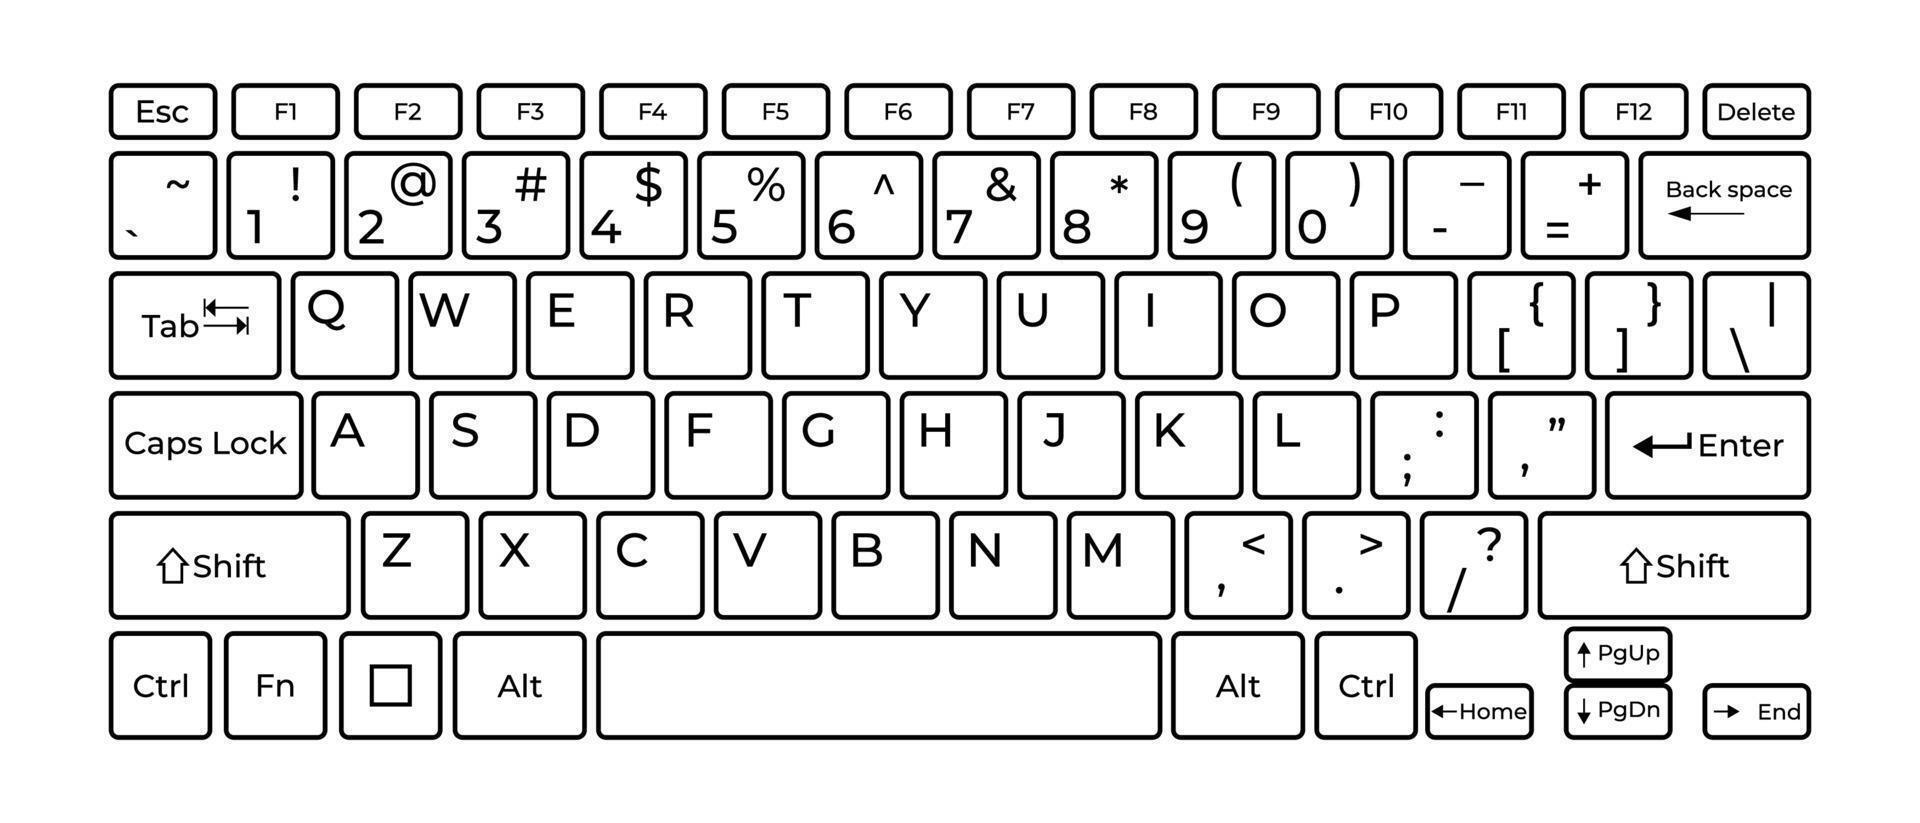
\includegraphics[width=0.7\textwidth]{Images/teclado.jpg}
    \caption{Imagen de un teclado}
    \label{fig:teclado}
\end{figure}
\subsection{Plataforma de despliegue}
Para el despliegue de la aplicación usaremos un ordenador que tenga XAMPP, ejecutado con Apache y MySQL, a partir de aqui, da un poco igual el SO, que usemos ya que la estructura es la misma, solamente necesitamos,
que el ordenador dónde se despliegue tenga bien las dependencias necesarias para poder ejecutar el programa.
\begin{figure}[ht]
    \centering
    
\includegraphics[width=0.7\textwidth]{Images/Xampp_logo.png}
    \caption{Imagen del logo de XAMPP}
    \label{fig:xampplogo}
\end{figure}
\clearpage
\subsection{Arquitectura logica}
Estructura del proyecto en el diagrama de clases:
\subsubsection{Diagrama de clases}

\begin{figure}[ht]
    \centering
    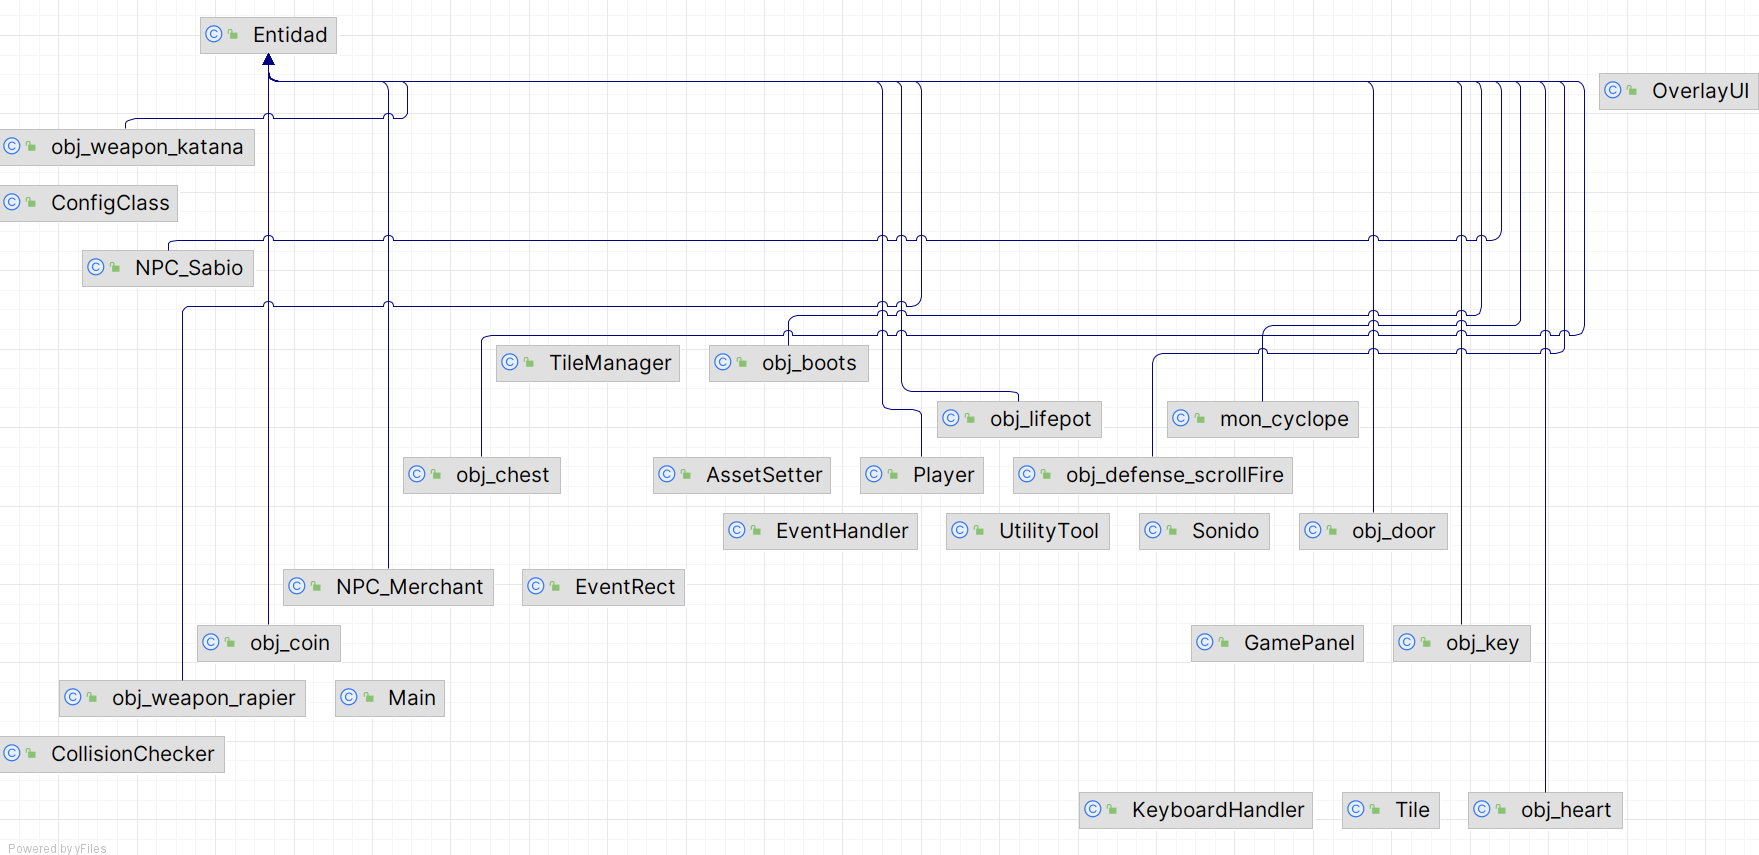
\includegraphics[width=1\textwidth]{Images/diagramadeclases.png}
    \caption{Diagrama de clases}
    \label{fig:diagrama-clases}
\end{figure}


\subsubsection{Explicaciones del diagrama}
Como podemos ver en el diagrama, hay varias clases importantes a lo largo de la estructura del mismo, que son, \textbf{Player, Gamepanel y Entidad}, estas clases son las más importantes ya que
nos ayudan a definir muchas cosas.\\
En el caso de \textit{Entidad}, nos permite desarrollar enemigos, objetos, npc y el propio jugador, ya que estos objetos, extienden de \textit{Entidad}, lo que deja que esta clase sea una clase llena de atributos.
\begin{flushright}
    \textit{Nota: No se han puesto los fields o atributos de cada clase en el diagrama debido a que Gamepanel y entidad cuentan con más de 20 atributos cada una y no permite ver el resto del diagrama}
\end{flushright}
\subsubsection{Metodo run}
En cuanto a \textit{Gamepanel}, esta clase sería la encargada de tener el panel de juego y conectarse con todas las clases del proyecto, ya que, por ejemplo define
el tamaño de los assetts, el tamaño del texto, y varios aspectos más de dentro del juego, esta clase además es de las más importantes ya que contiene parte de los métodos más críticos del proyecto como por ejemplo el siguiente.\\
\begin{figure}[ht]
    \centering
    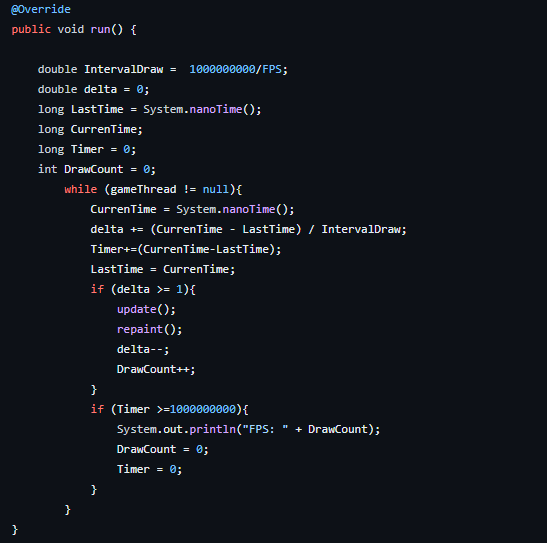
\includegraphics[width=0.7\textwidth]{Images/fpsMethod.PNG}
    \caption{Método del hilo principal}
    \label{fig:metodohiloprincipal}
\end{figure}
\\
Este método empieza inicializando 6 variables que le servirán para calcular un \textit{delta}, para ello hace uso de esta ecuación:
$$\text{IntervalDraw} = \frac{1}{\text{FPS}}$$
Como vemos esta ecuación sería la inversa de los \textit{FPS o Frames per Second}, dicho esto explicaremos cada variable.
\begin{itemize}
    \item \textit{IntervalDraw:} esta variable es la encargada de calcular en nanosegundos el tiempo necesario para dibujar un fotograma a la velocidad deseada
    \item \textit{delta:} Lleva un seguimiento del tiempo transcurrido desde el último fotograma.
    \item \textit{LastTime:} Almacena el tiempo en nanosegundos en el que se procesó el último fotograma.
    \item \textit{CurrenTime:} Almacena el tiempo actual en nanosegundos.
    \item \textit{Timer:} Lleva el seguimiento del tiempo transcurrido.
    \item \textit{DrawCount:} Es el contador de FPS del juego.
\end{itemize}
\textbf{Bucle principal}\\
Esta parte del codigo, ejecuta un bucle (El bucle se ejecuta mientras gameThread no sea nulo (es decir, mientras el juego esté funcionando)) en el cual ocurre lo siguiente:
\begin{itemize}
    \item Se actualiza el valor de CurrenTime.
    \item Se calcula el tiempo transcurrido desde el último fotograma y se agrega a delta.
    \item Se actualiza el valor de LastTime.
    \item Si delta supera 1, se llama a los métodos update() y repaint() para actualizar y dibujar el siguiente fotograma.
    \item Se decrementa delta en 1 y se incrementa DrawCount.
    \item Si Timer supera 1 segundo (1,000,000,000 nanosegundos), se muestra el número de fotogramas dibujados en la consola y se reinician los contadores.
\end{itemize}
Es decir, este metodo controla la lógica del dibujado o render del juego para que sea siempre de 60 fotogramas por segundo, es decir, dibuja 60 veces por segundo lo que tenemos en pantalla
de esta manera no tenemos valores extremadamente altos que no sirve de nada tener en un juego de este estilo, ya que no necesitamos que se dibuje todo 300 mil veces por segundo.\\

\clearpage
% ---------------------------------------
\subsubsection{Método loadmap}
Aun asi, vale la pena destacar varios métodos interesantes como el de \textit{"loadmap"}, que encontramos en la clase \textit{"TileMananger"}, la clase encargada de leer el mapa del juego.
\begin{figure}[ht]
    \centering
    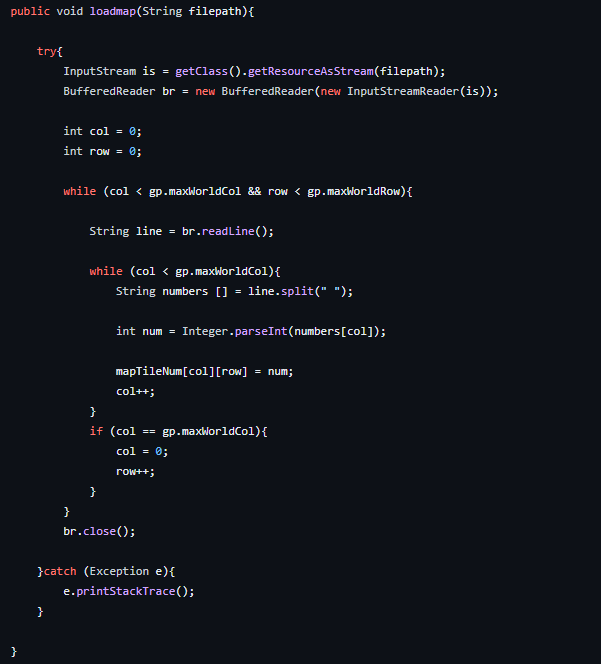
\includegraphics[width=0.7\textwidth]{Images/loadmap.PNG}
    \caption{Método de carga de mapas}
    \label{fig:metodocargademapa}
\end{figure}
\\
\textbf{Explicacion del metodo}\\
Este método funciona de la siguiente manera, a modo de resumen, lee el archivo .txt del mapa que esta compuesto solo de números y a cada número le asigna una casilla, de esta manera, según el número la casilla
tiene una imagen u otra.\\
Ahora de forma extensa, explicaremos paso por paso que hace este método:
\begin{enumerate}
    \item \texttt{El método toma una cadena, \textit{"filepath"}, esta cadena se refiere a la ubicación del mapa en el sistema de archivos del ordenador, es decir, la ruta del archivo}
    \item \texttt{InputStream is = getClass().getResourceAsStream(filepath); BufferedReader br = \\
              new BufferedReader(new InputStreamReader(is));
              esta parte del codigo lo que hace es crear un BufferReader que lee el archivo del mapa.}
    \item \texttt{"getClass().getResourceAsStream(filepath)" lo que hace es localizar el archivo en el sistema.}
    \item \texttt{Las variables \textit{row} y \textit{col} nos sirven para saber en que posición del mapa se encuentra.}
    \item \texttt{"while (col < gp.maxWorldCol \&\& row < gp.maxWorldRow)" el bucle continua mientras no se llegue al final del mapa}
    \item \texttt{"String line = br.readLine();" simplemente lee una linea del archivo}
    \item \texttt{"while (col < gp.maxWorldCol)" el bucle se ejecuta para cada columna actual}
    \item \texttt{"String numbers [] = line.split(" "); int num = Integer.parseInt(numbers[col]);\\ mapTileNum[col][row] = num; col++;" aquí se divide la línea en números, se convierte cada número a un entero y se almacena en el array \textit{mapTileNum}}
    \item \texttt{"if (col == gp.maxWorldCol){ col = 0; row++; }" Cuando se ha llegado al final de una fila, se incrementa la variable \textit{row} y se reinicia la variable \textit{col}}
    \item \texttt{"br.close();" cierra el BufferReader.}
    \item \texttt{Y por ultimo el catch captura la excepcion en caso de que se produzca}
\end{enumerate}
Este es un método muy curioso ya que puede producir otra excepción más que no he controlado, estamos hablando de la famosa excepción \textit{java.lang.OutOfMemoryError}, debido a que si tenemos un mapa muy grande
la máquina virtual de java, \textit{JVM} se queda sin memoria en el heap y detiene el programa porque ha "roto".
\clearpage
\subsubsection{Método draw}
Otro método interesante sería el método \textit{"draw"} de nuevo de la clase \textit{"TileMananger"}, el cual se encarga de dibujar las "casillas" de juego.\\
De forma resumida, va dibujando las casillas en la posición determinada en el mapa del juego.\\
\begin{figure}[ht]
    \centering
    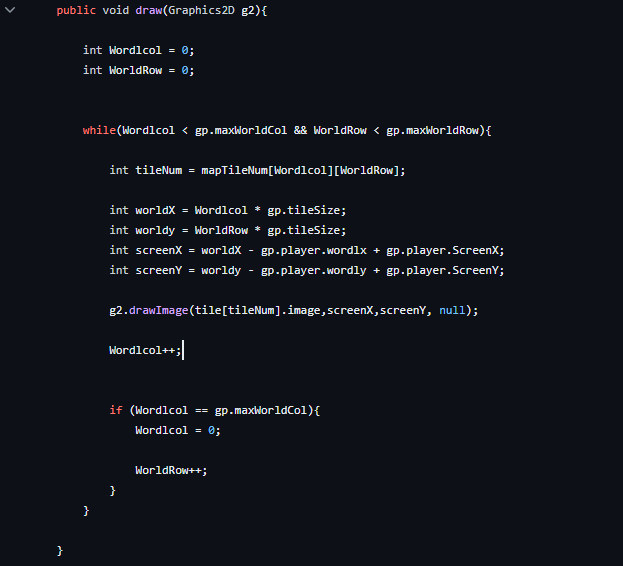
\includegraphics[width=0.6\textwidth]{Images/draw.PNG}
    \caption{Método de dibujado de mapas}
    \label{fig:metododibujadodemapa}
\end{figure}

\textbf{Explicación del método}\\
Este método es bastante simple de entender si hemos entendido los anteriores, por lo que procederemos a su desglose:
\begin{enumerate}
    \item \texttt{public void draw(Graphics2D g2) primero recibe un objeto del tipo Graphics2D como argumento que usará para dibujar en pantalla.}
    \item \texttt{worlCol y worlRow son las variables que usaremos para rastrear la posición en la que nos encontramos}
    \item \texttt{while(Wordlcol < gp.maxWorldCol \&\& WorldRow < gp.maxWorldRow) este bucle continua mientras no lleguemos al final del mapa}
    \item \texttt{int tileNum = mapTileNum[Wordlcol][WorldRow] y aqui obtenemos el número de la casilla que se va a dibujar}
    \item \texttt{int worldX = Wordlcol * gp.tileSize; int worldy = WorldRow * gp.tileSize} aquí calculamos las coordenadas \texttt{x} e \texttt{y} del juego
    \item \texttt{int screenX = worldX - gp.player.wordlx + gp.player.ScreenX; \\int screenY = worldy - gp.player.wordly + gp.player.ScreenY aqui se calculan las coordenadas de la pantalla}
    \item \texttt{g2.drawImage(tile[tileNum].image,screenX,screenY, null); aqui dibujamos la casilla}
    \item \texttt{Incrementamos las columnas de la variable que rastrea las columnas}
    \item \texttt{"if (Wordlcol == gp.maxWorldCol){ Wordlcol = 0; WorldRow++; }" cuando se ha llegado al final de una fila, se incrementa la variable WorldRow y se reinicia la variable Wordlcol}
\end{enumerate}



\clearpage
% ------------------------------------------------
\subsection{Diagrama de casos de uso}
En el diagrama de casos de uso, tenemos un actor que seria el jugador. Este actor realizaría varias funciones, como por ejemplo:
\begin{itemize}
    \item Empezar el juego
    \item Mover el personaje
    \item Pausar el juego
    \item Ver el estado del personaje
    \item Salir del juego
    \item Combatir
    \item Interactuar con NPCs
    \item Obtener objetos, experiencia, dinero.
    \item Interactuar con el entorno
    \item Leer de la base de datos
    \item Morir
\end{itemize}

\begin{figure}[ht]
    \centering
    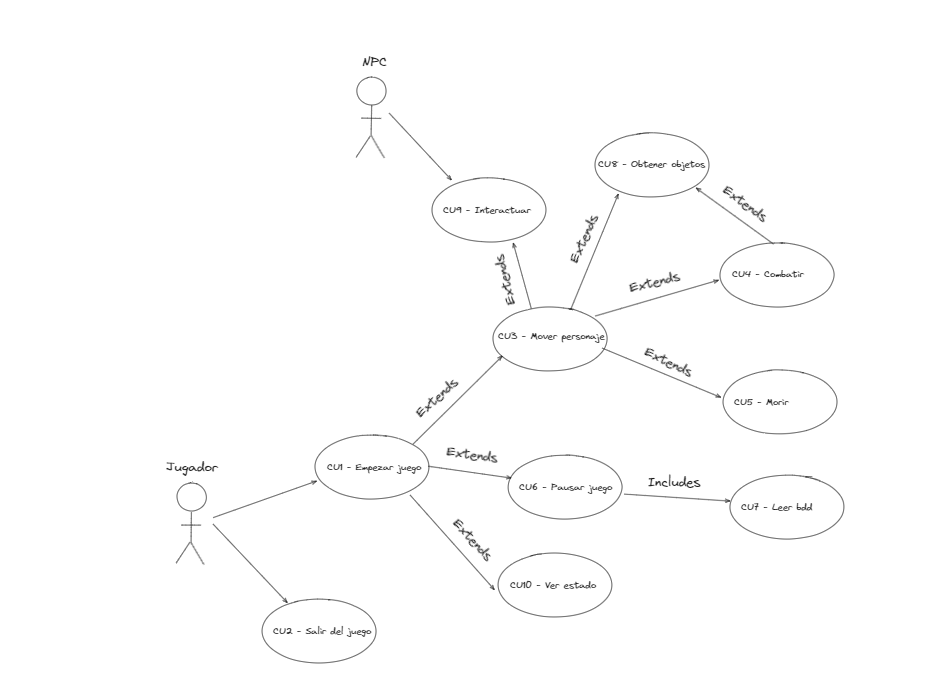
\includegraphics[width=0.6\textwidth]{Images/diagramaCU.PNG}
    \caption{Diagrama de casos de uso}
    \label{fig:diagramas}
\end{figure}

\clearpage
% -----------------------------------------------

\begin{table}[!ht]
    \centering
    \begin{tabular}{|c|p{12cm}|}
        \hline
        \textbf{Apartados}     & \textbf{CU1-Empezar juego}                                                                                                             \\
        \hline
        Precondiciones         & El programa debe estar en ejecución                                                                                                    \\
        \hline
        Postcondiciones        & El programa cambiará al estado de \textit{playstate} lo que provocará el cambio de interfaz gráfica                                    \\
        \hline
        Actor                  & Jugador                                                                                                                                \\
        \hline
        Descripción            & El jugador:
        \begin{enumerate}
            \item Mediante el movimiento del cursor con las teclas \textbf{W} y \textbf{S}, el actor colocará el cursor en la posición deseada
            \item Presionará la tecla \textbf{ENTER}, la cual aceptará la opción escogida, en este caso \textbf{Nuevo juego}
            \item El programa entrará en el \textit{playstate}
            \item Empezará el juego
        \end{enumerate}                               \\
        \hline
        Escenarios secundarios & \textbf{Escenario alternativo 1:}
        \begin{itemize}
            \item El jugador, estando en la pantalla de menú principal después de haber vuelto a la misma desde el menú de opciones del programa.
            \item Presiona de nuevo la tecla \textbf{ENTER} sobre la misma opción.
            \item[\faAngleRight] Provocaría la vuelta al \textit{playstate} y que los objetos vuelvan a estar donde estaban, así como npcs, enemigos y posición del jugador.
        \end{itemize} \\
        \hline
        Frecuencia de uso      & Baja                                                                                                                                   \\
        \hline
    \end{tabular}
    \caption{Caso de uso 1 - Empezar juego}
    \label{tab:casosdeuso01-table}
\end{table}

\begin{table}[!ht]
    \centering
    \begin{tabular}{|c|p{12cm}|}
        \hline
        \textbf{Apartados}     & \textbf{CU2-Salir del juego}                                                                                \\
        \hline
        Precondiciones         & El programa debe estar en funcionamiento                                                                    \\
        \hline
        Postcondiciones        & El programa, pararía su ejecución                                                                           \\
        \hline
        Actor                  & Jugador                                                                                                     \\
        \hline
        Descripción            & El jugador:
        \begin{itemize}
            \item Mediante el movimiento del cursor con las teclas \textbf{W} y \textbf{S}, el actor colocará el cursor en la posición deseada
            \item Presionará la tecla \textbf{ENTER}, la cual aceptará la opción escogida, en este caso \textbf{Salir}
            \item El programa terminaría su ejecución
            \item Se cerraría automáticamente
        \end{itemize}    \\
        \hline
        Escenarios secundarios & \textbf{Escenario alternativo 1:}
        \begin{itemize}
            \item El jugador, estando en la pantalla de menú principal después de haber vuelto a la misma desde el menú de opciones del programa.
            \item Presiona de nuevo la tecla \textbf{ENTER} sobre la misma opción.
            \item[\faAngleRight] Provocaría la parada de la ejecución del programa.
        \end{itemize} \\
        \hline
        Frecuencia de uso      & Baja                                                                                                        \\
        \hline
    \end{tabular}
    \caption{Caso de uso 2 - Salir del juego}
    \label{tab:casosdeuso2-table}
\end{table}

\begin{table}[!ht]
    \centering
    \begin{tabular}{|c|p{12cm}|}
        \hline
        \textbf{Apartados}     & \textbf{CU3-Mover personaje}                                                                 \\
        \hline
        Precondiciones         & El programa debe estar en \textit{playstate}, es decir \textbf{CU1}                          \\
        \hline
        Postcondiciones        & El programa cambiará la posición \textbf{X} o \textit{Y} del personaje con una animación     \\
        \hline
        Actor                  & Jugador                                                                                      \\
        \hline
        Descripción            & El jugador:
        \begin{itemize}
            \item Mediante las teclas \textbf{W,A,S,D}, presionará, una de ellas.
            \item Dependiendo de la tecla, el personaje del juego, se moverá en pantalla hacia 1 de las 4 direcciones posibles
            \item El personaje se moverá tanto tiempo como esté presionada la tecla elegida.
            \item El personaje parará su movimiento cuando se deje de presionar la tecla.
        \end{itemize}     \\
        \hline
        Escenarios secundarios & \textbf{Escenario alternativo 1:}
        \begin{itemize}
            \item El jugador colisiona contra un objeto, casilla y/o NPC.
            \item[\faAngleRight] Si el jugador avanza en la dirección de esta casilla, objeto o NPC, no se producirá el movimiento
        \end{itemize} \\
        \hline
        Frecuencia de uso      & Alta                                                                                         \\
        \hline
    \end{tabular}
    \caption{Caso de uso 3 - Mover personaje}
    \label{tab:casosdeuso3-table}
\end{table}

\begin{table}[!ht]
    \centering
    \begin{tabular}{|c|p{12cm}|}
        \hline
        \textbf{Apartados}     & \textbf{CU4-Combatir}                                                                                \\
        \hline
        Precondiciones         & El jugador se encuentra en el \textbf{CU1} previamente.                                              \\
        \hline
        Postcondiciones        & El jugador resta puntos de salud al enemigo.                                                         \\
        \hline
        Actor                  & Jugador                                                                                              \\
        \hline
        Descripción            & El jugador:
        \begin{itemize}
            \item Econtrándose en el \textbf{CU1}
            \item Haciendo uso del \textbf{CU3}
            \item Se encuentra con un \textit{enemigo}
            \item[\faAngleRight] Puede combatir
            \item Le restará puntos de salud al \textit{enemigo} con un ataque en caso de acierto
            \item El \textit{enemigo}, tendrá un tiempo en el que será invulnerable
            \item Esos puntos de salud se verán representados por una barra de puntos de salud que se colocará encima del \textit{enemigo}
            \item[\faAngleRight] Cuando los puntos de salud llegan a cero o menos de cero puntos, el \textit{enemigo}, desaparece
        \end{itemize} \\
        \hline
        Escenarios secundarios & \textbf{Escenario alternativo 1:}
        \begin{itemize}
            \item El jugador colisiona contra el enemigo.
            \item[\faAngleRight] Si el jugador colisiona contra el enemigo, perderá puntos de salud
            \item El jugador además si es dañado, tendrá un tiempo en el cual será invulnerable
        \end{itemize}
        \textbf{Escenario alternativo 2:}
        \begin{itemize}
            \item El jugador pierde todos sus puntos de salud
            \item Esto provocaría el \textbf{CU5}
            \item El programa estaría en el \textit{gameoverstate}
        \end{itemize}                                                                         \\
        \hline
        Frecuencia de uso      & Media                                                                                                \\
        \hline
    \end{tabular}
    \caption{Caso de uso 4 - Combatir}
    \label{tab:casosdeuso4-table}
\end{table}

\begin{table}[!ht]
    \centering
    \begin{tabular}{|c|p{12cm}|}
        \hline
        \textbf{Apartados}     & \textbf{CU5-Morir}                                                                                              \\
        \hline
        Precondiciones         & El jugador ha recibido daño o ha experimentado algo que haya restado sus puntos de salud a cero o menos de cero \\
        \hline
        Postcondiciones        & El programa pasa a \textit{gameoverstate}, además aparecerá la interfaz gráfica de la pantalla de fin de juego  \\
        \hline
        Actor                  & Jugador                                                                                                         \\
        \hline
        Descripción            & El jugador:
        \begin{itemize}
            \item Dentro del \textbf{CU1}
            \item Ve mermados sus puntos de salud a cero o menos de cero
            \item[\faAngleRight] Provoca su muerte
            \item[\faAngleRight] Aparece una pantalla de fin de juego con dos opciones
            \item Puede elegir si volver a intentarlo o salir, mediante las teclas \textbf{W} y \textbf{S}
            \item El jugador seleccionaría una opción con la tecla \textbf{ENTER}
        \end{itemize}                                            \\
        \hline
        Escenarios secundarios & \textbf{Escenario alternativo 1:}
        \begin{itemize}
            \item El jugador ha escogido la opción de volver a intentarlo o \textit{retry}
            \item Devuelve el personaje a su posición inicial
            \item También a los enemigos, NPCs y objetos
        \end{itemize}
        \textbf{Escenario alternativo 2:}
        \begin{itemize}
            \item El jugador selecciona la opción de salir
            \item Devuelve al jugador a la pantalla de menú principal
            \item Cambia el estado del programa a \textit{TitleScreenstate}
        \end{itemize}                                                                           \\
        \hline
        Frecuencia de uso      & Baja                                                                                                            \\
        \hline
    \end{tabular}
    \caption{Caso de uso 5 - Morir}
    \label{tab:casosdeuso5-table}
\end{table}

\begin{table}[!ht]
    \centering
    \begin{tabular}{|c|p{12cm}|}
        \hline
        \textbf{Apartados} & \textbf{CU6-Pausar el juego}                                                     \\
        \hline
        Precondiciones     & Debemos estar en el \textbf{CU1}                                                 \\
        \hline
        Postcondiciones    & El programa pasa a estar en estado \textit{pauseState} y provoca el \textbf{CU7} \\
        \hline
        Actor              & Jugador                                                                          \\
        \hline
        Descripción        & El jugador:
        \begin{itemize}
            \item Dentro del \textbf{CU1}
            \item El jugador presiona la tecla \textbf{P}
            \item El programa esta en \textit{pauseState}
            \item[\faAngleRight] Se abre una ventana emergente dentro del programa, el menú de pausa
            \item[\faAngleRight] Provoca el \textbf{CU7}
            \item[\faAngleRight] Lista objetos directamente de la base de datos
            \item Si el jugador presiona de nuevo la tecla \textbf{P}, volvería de nuevo al \textit{gamestate}
        \end{itemize}     \\
        \hline
        Frecuencia de uso  & Alta                                                                             \\
        \hline
    \end{tabular}
    \caption{Caso de uso 6 - Pausar el juego}
    \label{tab:casosdeuso6-table}
\end{table}

\begin{table}[!ht]
    \centering
    \begin{tabular}{|c|p{12cm}|}
        \hline
        \textbf{Apartados}     & \textbf{CU7-Leer la base de datos}                                           \\
        \hline
        Precondiciones         & Estar conectado a la base de datos y estar en el \textbf{CU6}                \\
        \hline
        Postcondiciones        & Realiza la lectura de datos sobre la base de datos y la muestra en pantalla  \\
        \hline
        Actor                  & Jugador                                                                      \\
        \hline
        Descripción            & El jugador:
        \begin{itemize}
            \item Estando en el \textbf{CU6}
            \item[\faAngleRight] Se muestra por pantalla un listado de objetos guardados en la base de datos
        \end{itemize}       \\
        \hline
        Escenarios secundarios & \textbf{Escenario alternativo 1:}
        \begin{itemize}
            \item El programa no es capaz de conectarse a la base de datos
            \item El programa por la consola, lanzará un mensaje de que no ha podido conectarse a la base de datos
            \item No parará la ejecución del mismo, y no mostrará el listado de objetos
        \end{itemize} \\
        \hline
        Frecuencia de uso      & Alta                                                                         \\
        \hline
    \end{tabular}
    \caption{Caso de uso 7 - Leer de la base de datos}
    \label{tab:casosdeuso7-table}
\end{table}

\begin{table}[!ht]
    \centering
    \begin{tabular}{|c|p{12cm}|}
        \hline
        \textbf{Apartados} & \textbf{CU8-Obtener Objetos}                        \\
        \hline
        Precondiciones     & Estar en el \textbf{CU1} y realizar el \textbf{CU3} \\
        \hline
        Postcondiciones    & Se añade el objeto al inventario del personaje      \\
        \hline
        Actor              & Jugador                                             \\
        \hline
        Descripción        & El jugador:
        \begin{itemize}
            \item Dentro del \textbf{CU1}
            \item Colisiona con un objeto al realizar el \textbf{CU3}
            \item El objeto desaparece
            \item Aparece un mensaje en la parte izquierda de la pantalla
            \item[\faAngleRight] Indica la obtención del objeto
            \item[\faAngleRight] El objeto es añadido al inventario del personaje
        \end{itemize}    \\
        \hline
        Frecuencia de uso  & Media                                               \\
        \hline
    \end{tabular}
    \caption{Caso de uso 8 - Obtener objetos}
    \label{tab:casosdeuso8-table}
\end{table}

\begin{table}[!ht]
    \centering
    \begin{tabular}{|c|p{12cm}|}
        \hline
        \textbf{Apartados}     & \textbf{CU9-Interactuar}                                                    \\
        \hline
        Precondiciones         & El jugador debe presionar la tecla \textbf{ENTER} tocando el NPC            \\
        \hline
        Postcondiciones        & El programa pasa a estar en estado de \textit{dialogueState}                \\
        \hline
        Actor                  & Jugador                                                                     \\
        \hline
        Descripción            & El jugador:
        \begin{itemize}
            \item Dentro del \textbf{CU1}
            \item Tocando el NPC
            \item Presiona la tecla \textbf{ENTER}
            \item[\faAngleRight] Se muestra un cuadro de dialogo en la parte superior de la pantalla
            \item[\faAngleRight] El programa estando en \textit{dialogueState} mantiene el resto del mundo parado
            \item Debe presionar \textbf{ENTER} para volver al \textit{playstate}
        \end{itemize} \\
        \hline
        Escenarios secundarios & \textbf{Escenario alternativo 1:}
        \begin{itemize}
            \item El jugador puede interactuar con ciertas casillas especiales
            \item Al interactuar con ellas se vuelve al \textit{dialogueState}
            \item Esta vez, esta interacción proporciona algo más que un dialogo
            \item El \textit{Healing pool Event} puede ser activado con este caso de uso
            \item Provocaría la recuperación de puntos de salud del personaje
        \end{itemize}                          \\
        \hline
        Frecuencia de uso      & Media                                                                       \\
        \hline
    \end{tabular}
    \caption{Caso de uso 9 - Interactuar}
    \label{tab:casosdeuso9-table}
\end{table}

\begin{table}[!ht]
    \centering
    \begin{tabular}{|c|p{12cm}|}
        \hline
        \textbf{Apartados} & \textbf{CU10-Ver estado}                                                                      \\
        \hline
        Precondiciones     & El jugador debe estar en el \textbf{CU1} y presionar la tecla \textbf{C}                      \\
        \hline
        Postcondiciones    & El jugador verá en la pantalla del programa una nueva interfaz gráfica con datos de interés   \\
        \hline
        Actor              & Jugador                                                                                       \\
        \hline
        Descripción        & El jugador:
        \begin{itemize}
            \item Estando en el \textbf{CU1}
            \item Presionará la tecla \textbf{C}
            \item[\faAngleRight] Provocará la aparición de una nueva interfaz gráfica con datos de interés acerca del personaje
            \item[\faAngleRight] Cambiará el estado del programa a \textit{statusState}
            \item[\faAngleRight] Podrá seleccionar otra arma dentro de su inventario
            \item[\faAngleRight] Moverá el cursor del inventario con las teclas \textbf{W,A,S,D}
            \item[\faAngleRight] Seleccionará el arma elegida con la tecla \textbf{ENTER}
            \item Cerrará esta interfaz con la tecla \textbf{C}
        \end{itemize} \\
        \hline
        Frecuencia de uso  & Media                                                                                         \\
        \hline
    \end{tabular}
    \caption{Caso de uso 10 - Ver estado}
    \label{tab:casosdeuso10-table}
\end{table}

\clearpage
\subsection{Historia del videojuego}
En esta parte explicaremos la breve narrativa, con la que cuenta el videojuego, tampoco hemos intentado hacer una narrativa super profunda, ya que requeriría de muchos más elementos
los cuales por falta de tiempo no podríamos añadir.\\
El videojuego transcurre en una época medieval, dentro de un mundo de fantasía, Eldoria, dentro de este mundo existe una gema que es capaz de realizar muchas acciones divinas, por ejemplo
curar enfermedades, provocar lluvia, otorgar suerte a una persona u entidad, etc \dots \\
Dentro del mundo hace relativamente poco, esta piedra mágica se ha perdido, y ahí es donde entra nuestro protagonista, el \textit{Ninja Rojo}, el cual se encargará de buscarla, ya que
si acaba en las manos equivocadas, sería algo terrible, pues igual que puede servir para el bien, también concede poderes para el mal.\\
De forma resumida sería la historia planeada para el videojuego, cabe destacar que por ejemplo una propuesta de mejora, sería ampliar este apartado algo más, meter más personajes, etc \dots

\clearpage

% -------------------------------------------------
\subsection{Pantallas del juego}
Dentro de esta sección hablaremos de las pantallas que hemos desarrollado en el juego, es decir, el menú principal, el inventario, por ejemplo.\\
Primero empezaremos con la pantalla del menú principal en la cual encontramos varios elementos.\\
\begin{figure}[!ht]
    \centering
    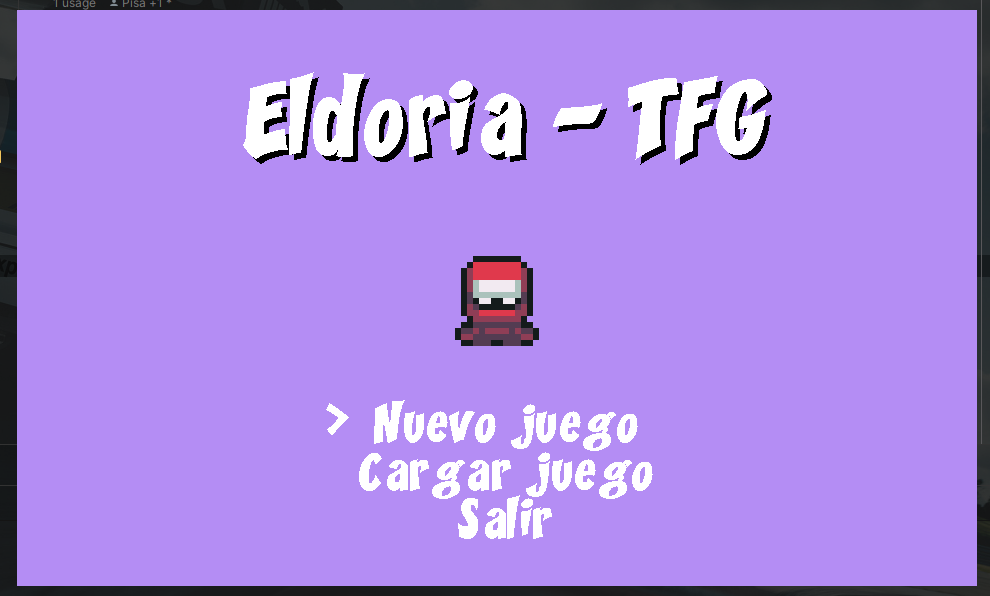
\includegraphics[width=0.6\textwidth]{Images/pantalla1tfg.png}
    \caption{Pantalla menu principal}
    \label{fig:pantalla1}
\end{figure}
Para empezar, tenemos que tener en cuenta que esta pantalla se dibuja con el método \textit{drawTitleScreen}, este método, nos permite crear la pantalla del menú. A continuación, lo primero de lo que hablaremos es del título de la pantalla
es decir, como vemos tiene una especie de sombreado, esto se consigue dibujando el texto primeramente en negro y despues en blanco movido un poco a la derecha, también, si nos fijamos en el centro de la pantalla observamos que tenemos una imagen del jugador,
esto aunque no sea de este propio apartado se puede tener en cuenta para futuras versiones, por ejemplo al seleccionar un personaje determinado, que aparezca en esta pantalla de título. Por último, vemos las opciones del juego, la primera es para cargar el juego, es decir
iniciarlo desde cero, la segunda es cargar juego, a dia de hoy no tenemos sistema de guardado de partida por archivos o similar por lo que esta opción se ha dejado escrita para futuras actualizaciones. Por último tenemos la opción de salir, que cierra la ventana del programa y termina su ejecución.\\

\begin{figure}[!ht]
    \centering
    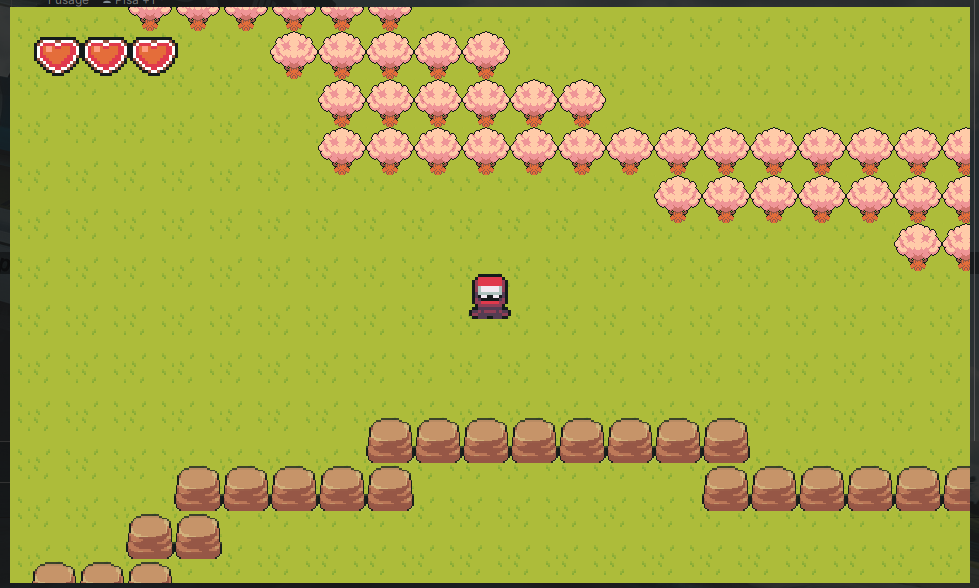
\includegraphics[width=0.6\textwidth]{Images/pantalla2tfg.png}
    \caption{Pantalla de juego}
    \label{fig:pantalla2}
\end{figure}
La segunda pantalla a analizar es la pantalla de juego, en ella transcurse todo el programa realmente, tenemos un panel que sigue al jugador allá donde vaya, y que nos muestra los enemigos, npc y casillas del mapa, esta pantalla además cuenta con una variación que es la pantalla con inventario, esta pantalla nos muestra al lado izquierdo las estadísticas del jugador, y a otro lado el inventario del mismo con descripciones para cada objeto.
Por otro lado, dentro de esta pantalla también observamos los corazones de vida del jugador.\\
\begin{figure}[!ht]
    \centering
    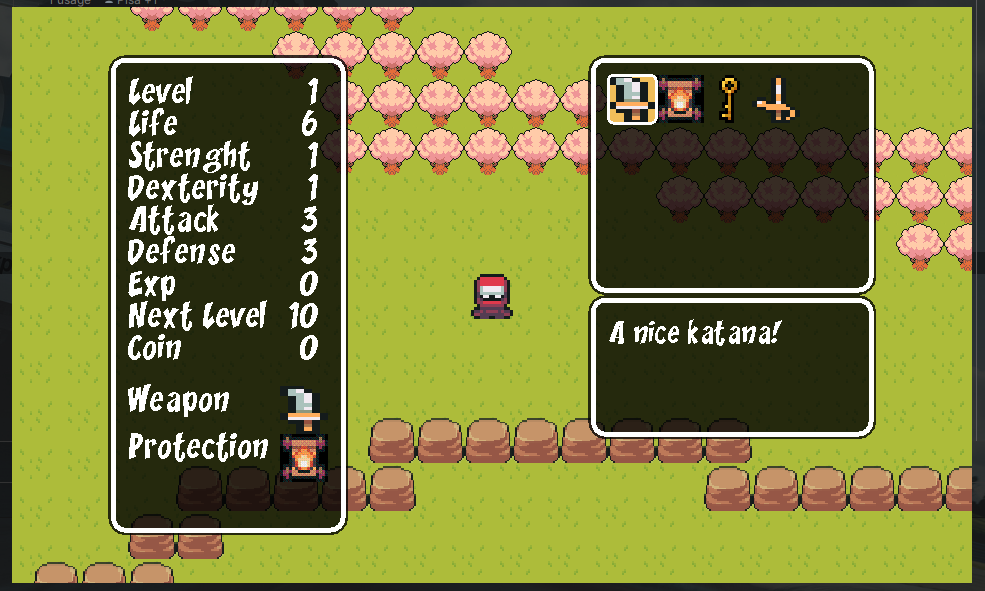
\includegraphics[width=0.6\textwidth]{Images/pantalla3tfg.png}
    \caption{Pantalla de inventario}
    \label{fig:pantalla3}
\end{figure}
Esta sería la pantalla referente al inventario, de la que hemos hablado anteriormente, en esta pantalla, lo que tenemos son varios cuadros que nos otorgan informacion sobre el personaje, esta pantalla la podemos dividir en 3 partes,
la primera parte es la del panel izquierdo que nos habla de las estadísticas, no tiene mucho misterio, simplemente nos muestra las estadísticas del jugador y una imagen del arma actual y el escudo o pergamino actual, el segundo panel sería el inventario en si, que es el panel derecho grande,
este panel cuenta con un cursor y un dato curioso, los objetos que sean armas, una vez seleccionados, cambia el fondo del inventario a un color amarillo, como se ve en la imagen, este panel es navegable, es decir, podemos seleccionar objetos con el cursor que vemos en pantalla. Por último tenemos el panel de descripción,
se trata del panel derecho que se encuentra en la posición más baja, este panel se ocupa de mostrar un breve texto a modo de descripción acerca del objeto sobre el que el cursor está encima.\\
\begin{figure}[!ht]
    \centering
    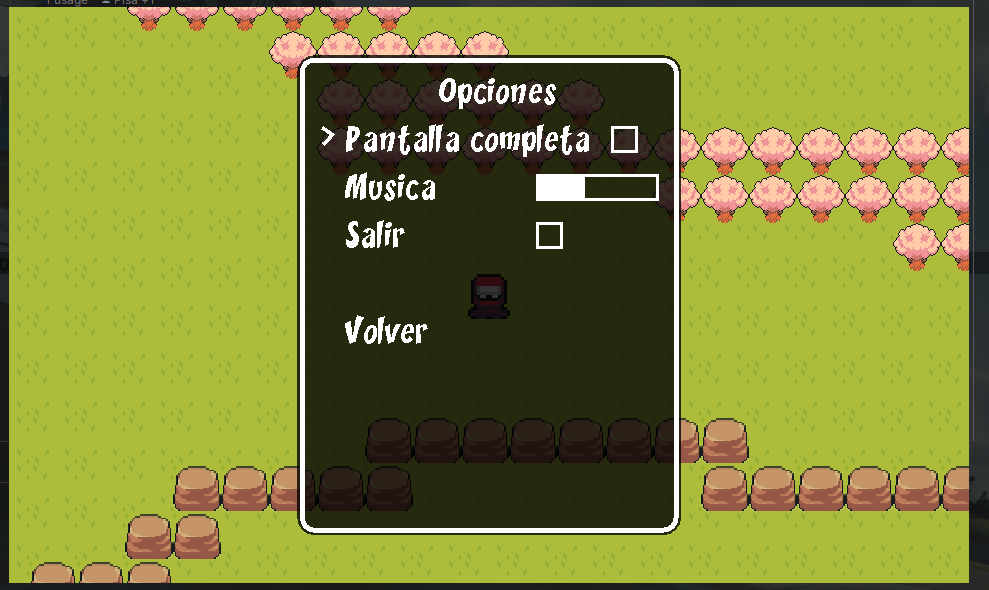
\includegraphics[width=0.6\textwidth]{Images/pantalla4tfg.png}
    \caption{Pantalla de opciones}
    \label{fig:pantalla4}
\end{figure}
Continuamos con la pantalla de opciones, en esta pantalla, lo que tenemos es lo siguiente, un recuadro en el que disponemos un título, despues varias opciones, con cuadrados, que los usamos a modo de checkbox, la primera opción, es la de pantalla completa, al darle a la tecla ENTER, se escribe automáticamente en el archivo
config.txt en la primera linea On, esto hace que cuando el programa lea nada más arrancar el archivo vea que la opción, está activada, así el programa iniciaría en el modo de pantalla completa. La siguiente opción, sería relativa al volumen de la música de fondo, este controlador, por llamarlo de alguna manera, sube el volumen en una escala
de 0 a 4, gracias a un cálculo producido en la clase \textit{Sonido} que tenemos dentro del proyecto, además dependiendo del volumen que dejemos escogido, en config.txt aparecerá en la segunda fila un número u otro, según el volumen. La última opción sería relativa a volver al menú principal, con esta opción iríamos a otra pantalla en la que podemos seleccionar si queremos ir al menú o no,
actualmente estamos trabajando para que funcione bien la selección ya que de momento solo podemos escoger la opción del sí. Por último y no por ello, menos importante la opción de volver, esta opción cerraría este marco y nos devolvería al estado de juego.\\
\begin{figure}[!ht]
    \centering
    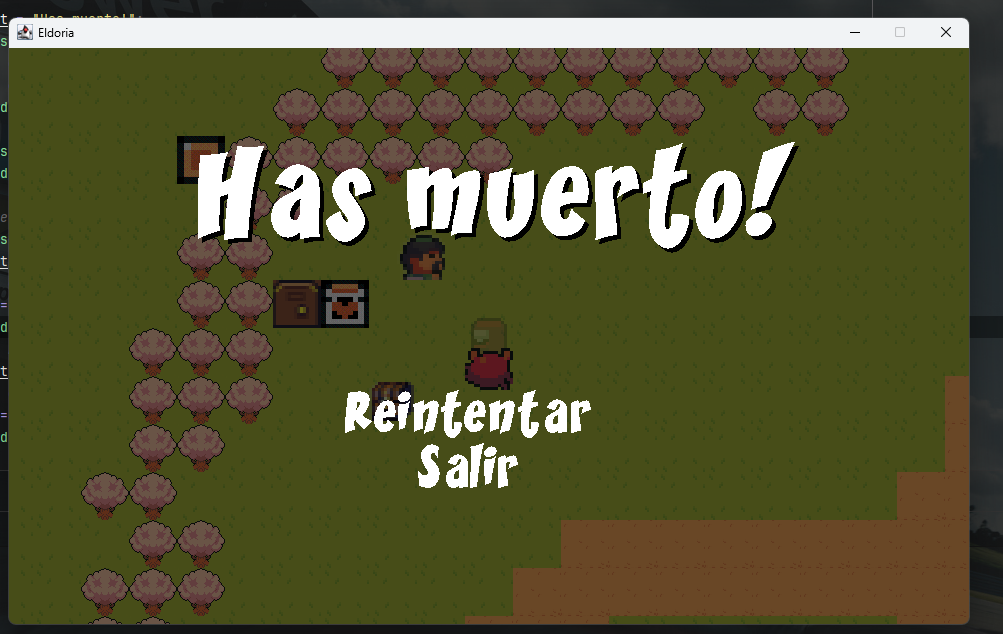
\includegraphics[width=0.6\textwidth]{Images/pantalla5tfg.png}
    \caption{Pantalla de Fin de juego}
    \label{fig:pantalla5}
\end{figure}
Una de las pantallas más importantes, la pantalla de fin de juego o \textit{game over} como les gusta decir a los jugadores, esta pantalla aparace,  no es una pantalla que el jugador pueda activar con una tecla o seleccionando una opción, aparece, cuando la vida del jugador llega a cero, y nos provee de dos opciones,
reintentar, que nos devuelve a la posición inicial y al principio del juego, o salir, que nos devuelve al menú principal.\\
\begin{figure}[!ht]
    \centering
    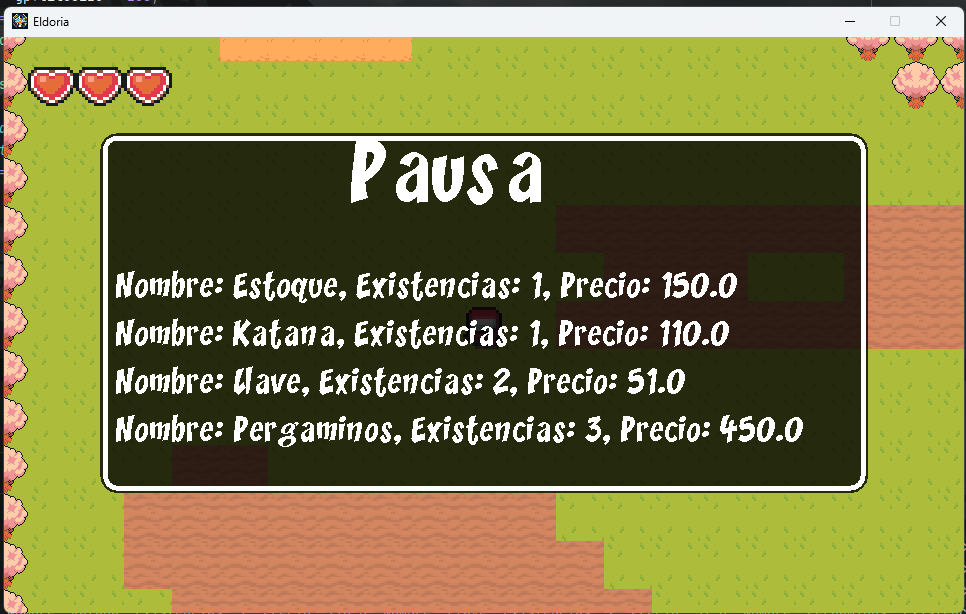
\includegraphics[width=0.6\textwidth]{Images/pantalla6tfg.png}
    \caption{Pantalla de Pausa y listado}
    \label{fig:pantalla6}
\end{figure}
La última pantalla que veremos es la pantalla de pausa que introduce el concepto de base de datos, en este caso hemos optado por poner un listado simple de objetos, aunque para un trabajo de futuro se podría hacer un listado interactivo que cuente el progreso del jugador, o que diga que objetos se nos han escapado durante la aventura.

\clearpage
% -------------------------------------------------
\section{Desarrollo realizado}
Para el desarrollo del proyecto hemos usado las siguientes herramientas:
\begin{itemize}
    \item IntelliJ
    \item XAMPP
    \item JDBC
    \item JDK 21
    \item Visual studio Code
    \item \LaTeX
    \item Excalidraw
    \item Github Repositories
    \item MySQL
\end{itemize}
Antes de comenzar la explicación del código pasaremos a explicar conceptualmente que hace el programa entero, ya que de esta manera, entenderemos mejor el código.
\subsection{Detalles conceptuales}
Este programa, sigue una filosofía clásica en cuestión al desarrollo del código, es decir, un videojuego, no deja de ser un hilo en bucle constante hasta que el jugador decide salir del juego o pararlo, en este caso hemos jugado con eso, y por ejemplo al ir entre
diferentes pantallas, en vez de usar otro hilo, lo cual podría generar interbloqueos o condiciones de carrera, hemos optado por crear estados, en los cuales, definimos ciertas condiciones y prohibiciones al jugador, durante los mismos, por ejemplo en el estado de pausa,
no se permite mover el personaje al jugador, en el estado de fin de juego, lo mismo, además que dependiendo del estado, ciertas teclas que antes funcionaban para mover el personaje, ahora servirían para mover el cursor de selección.\\
También hay que tener en cuenta que este videojuego, se ejecuta sin motor de juego[1], es decir, esto tiene una gran ventaja y desventaja al mismo tiempo. La principal ventaja es un \textbf{mayor control y flexibilidad} a la hora de desarrollar funciones referentes al juego, el problema, es
que esto añade \textbf{complejidad y tiempo de desarrollo} comparado con otros motores como \textit{Unity, Unreal Engine, Godot}, por ejemplo.\\
La pregunta del millón, ¿Cómo funcionan las colisiones?, es una pregunta que se ha realizado durante la primera fase del desarrollo, como hacemos las colisiones dentro de este juego, pero primero debemos explicar, a que nos referimos con las colisiones.
Con colisiones nos referimos a la \textit{hitbox}, una hitbox es una caja invisible que se utiliza en los videojuegos para detectar colisiones y registrar impactos entre objetos dentro del juego. Dentro del desarrollo lo que hemos hecho ha sido con \textit{swing}, desarrollar un cuadrado invisible,
alrededor de los personajes y NPCs, que al entrar en contacto con otro cuadrado, no pueda moverse en las coordenadas x o y, esto de igual manera afectaría a casillas como por ejemplo la de los árboles, el problema de esto es que debemos hacer una \textit{hitbox común} en caso de tener las mismas dimensiones,
con todos los personajes, o una \textit{hitbox} personalizada, en caso de tener personajes de varias dimensiones diferentes, un equivalente en \textit{Unity}, sería el \textit{Box collider}, en ese motor, gracias a esa opción, podemos desarrollar una hitbox personalizada que se adiere al \textit{GameObject} al que le hayamos,
puesto esta opción.\\
\begin{flushright}
    [1]\textit{Un motor de juego es un software que proporciona un conjunto de herramientas y funcionalidades básicas necesarias para desarrollar videojuegos.}
\end{flushright}


\clearpage
% --------------------------------------------------
Ahora pasaremos a explicar el código de una manera más detallada, parándonos un poco más clase por clase para explicar lo que hemos desarrollado.
\subsection{Detalles del codigo desarrollado}
Empezaremos describiendo lo que realiza la clase principal, la clase \textit{"Main"}, cuyo código es:
\begin{lstlisting}
    package main;
    import javax.imageio.ImageIO;
import javax.swing.*;
import java.awt.*;
import java.io.IOException;

public class Main {
    public static JFrame win;
    public static void main(String args[]){
        win = new JFrame();
        win.setDefaultCloseOperation(JFrame.EXIT_ON_CLOSE);
        win.setResizable(false);
        win.setTitle("Eldoria");

        try {
            Image icon = ImageIO.read(Main.class
                                .getResource("/player/icono.jpg"));
            win.setIconImage(icon);
        } catch (IOException e) {
            e.printStackTrace();
        }

        GamePanel gpanel = new GamePanel();
        win.add(gpanel);

        gpanel.config.loadConfig();
        if (gpanel.fullScreenOn == true){
            win.setUndecorated(true);
        }

        win.pack();

        win.setLocationRelativeTo(null);
        win.setVisible(true);
        gpanel.setupStuff();
        gpanel.startGameThread();

    }
}
\end{lstlisting}
Dentro de este código encontramos varios aspectos a destacar, el primero es que estamos creando un JFrame en primera instancia y luego le estamos diciendo tambien que al darle a la "X", nos cierre el programa automaticamente.
Continuamos diciéndole que no queremos un resize de la ventana actual del juego, por eso el false, seguimos con el titulo, y a continuacion la instancia de GamePanel, la cual nos servirá para instanciar más cosas.
Centramos la ventana con el setLocationRelativeTo, la hacemos visible y le decimos a GamePanel que vaya dibujando ciertas cosas del videojuego e inicie el hilo principal del juego.\\

Yendo más a fondo, en la parte del try lo que le cargamos al programa es el icono del mismo, queremos que exista un icono en la aplicación, por lo que lo realizamos bajo un try and catch, ya que puede producir una excepción,
después de agregar el gpanel, lo que hacemos es saber si el juego está configurado con la pantalla completa, para ello cargamos la configuración del archivo config.txt, si la pantalla completa está en true, quitamos los bordes de la pantalla.\\

Continuamos la explicación con la clase \textit{"Gamepanel"}, la cual es la encargada de realizar varias acciones principales dentro de la aplicación, si bien es cierto que hemos explicado algún método ya, explicaremos el resto
que no son tan importantes pero igualmente son interesantes de saber.\\
\begin{lstlisting}
    public void setupStuff(){
        aSetter.setObject();
        aSetter.setNPC();
        aSetter.setMonster();
        playMusic(1);
        gameState = titleState;
    }
\end{lstlisting}
Este método es el que se encarga de poner todo a punto en el \textit{"tablero de juego"}, como vemos, llama al metodo setObject, setNpc, setMonster, y playMusic, los cuales se encargan respectivamente
de poner los objetos en el mapa, los npc, los monstruos y reproducir la música de fondo, por último se cambia la variable de gamestate que es con la que se jugará dentro del código para poner el juego en pausa, o
en el menú principal, por ejemplo.\\
Continuamos con un método que actualmente no es de está manera pero aun así es interesante de ver ya que ha servido de base para futuras versiones, y es el método paintComponent antes de realizar la función de tener el juego
en pantalla completa:
\begin{lstlisting}
    public void paintComponent(Graphics g){

    super.paintComponents(g);
    Graphics2D g2 = (Graphics2D)g;
    g2.setColor(Color.BLACK);
    g2.fillRect(0, 0, getWidth(), getHeight());

    //Title screen
    if (gameState == titleState){
        overlayUI.drawUI(g2);
    }
    //Others
    else {
        ///casillas
        TileM.draw(g2);
        //Adicion de entidades a la lista
        entidadList.add(player);
        for (int i = 0; i<npc.length; i++){
            if (npc[i] != null){
                entidadList.add(npc[i]);
            }
        }
        for (int i=0; i<obj.length; i++){
            if (obj[i]!= null){
                entidadList.add(obj[i]);
            }
        }
        for (int i=0; i<monster.length; i++){
            if (monster[i]!= null){
                entidadList.add(monster[i]);
            }
        }
        /// ordenado
        Collections.sort(entidadList, new Comparator<Entidad>() {
            @Override
            public int compare(Entidad o1, Entidad o2) {
                int result = Integer.compare(o1.wordly, o2.wordlx);
                return 0;
            }
        });

        //Draw entity
        for (int i = 0; i<entidadList.size(); i++ ){
            entidadList.get(i).draw(g2);
        }

        /// Empty entity list
        entidadList.clear();


        //Overlay UI
        overlayUI.drawUI(g2);

    }
    g2.dispose();
}
\end{lstlisting}
Para empezar, este método sería el encargado de pintar todos los componentes en la pantalla, es decir, pinta las casillas y el fondo del juego sobre el que se pondrán las imágenes usadas para el juego,
también se encarga de dibujar o renderizar, los monstruos, npcs, y el personaje. Profundizaremos más en ello.\\
Lo primero que realiza, después de coger los 4 parámetros que coge, es cerciorarse del gameState en el que nos encontramos, al hacerlo dibujará la pantalla de título o la de juego, en caso de estar en la
de titulo, lo que encontramos es una llamada a la clase encargada de la \textit{User Interface}, la hemos llamado \textit{OverlayUI}, ya que no deja de ser lo que se conoce tipicamente en imagen como overlay,
y UI debido a que se trata de la interfaz de usuario. Si seguimos, en caso de no estar en el estado de pantalla de titulo, lo que haría el código es seguir por la parte del \textit{else}, en este parte el código empieza
dibujando las casillas con el ".draw", y continua añadiendo las entidades al juego, en este programa como todas las entidades las guardamos en listas, tenemos que realizar un bucle for que nos permita recorrer la lista
que contiene las entidades. Al acabar llegamos a la parte que ordena las entidades con la interfaz \textit{Comparator}, sobreescribimos el método de esta interfaz para ordenadr las entidades y continuamos con el código.
Una vez que tenemos ordenadas las entidades, lo que hará el código es dibujar las propias entidades, ordenadas en función de donde aparece el jugador, cuanto más cerca más prioridad tiene de ser dibujada la entidad.
por último limpiamos la lista de entidades \textit{temporales} y con todo puesto, le decimos a la clase del Overlay, que lo dibuje todo, y para acabar, metemos un .dispose, para acabar. \\
Antes de realizar la funcionalidad de tener el juego en pantalla completa, se realizaba el dibujado de esa manera, actualmente, seguimos usando el mismo método salvo que cuenta con una variación, la cual es que hemos eliminado,
varias instancias de g2, es decir del objeto de Graphics2D, esto es debido a que para mostrar el juego en la pantalla completa el juego lo que realiza es lo siguiente:\\
\begin{figure}[ht]
    \centering
    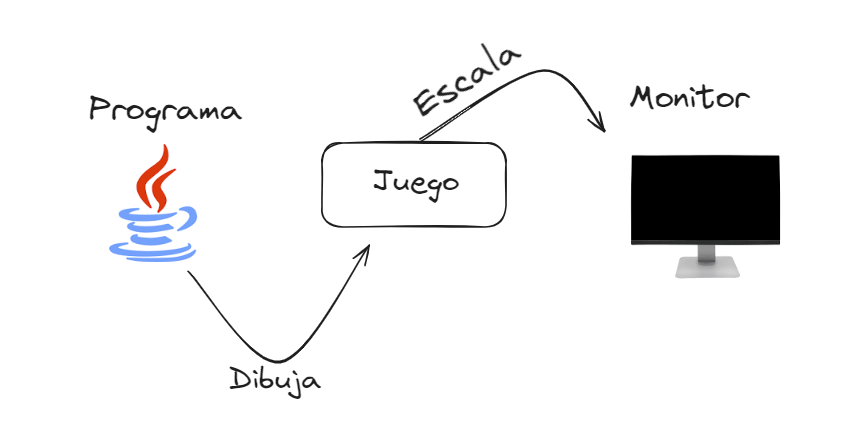
\includegraphics[width=0.6\textwidth]{Images/Fullscrennmode.PNG}
    \caption{¿Cómo dibuja el programa la pantalla completa?}
    \label{fig:fullscreenmode}
\end{figure}
Esto es importante tenerlo en cuenta ya que después de ser dibujado el juego, necesita ser escalado a la resolución de nuestro monitor, en las primeras fases del desarrollo, se realizó el juego en un formato de 4:3,
formato clásico de monitores más bien modestos o antiguos, según se implementó la función de pantalla completa, se ha tenido que cambiar lo que se conoce como \textit{aspect ratio} a uno más actual y más usado, como puede
ser el formato de 16:9, algo más estirado que el clásico 4:3, esto permite que se pueda mostrar el juego en monitores de 1920x1080 pixeles, o tambien en monitores 4K, de resolución 3840x2160 pixeles. ¿Por qué es importante saber esto?
esto es crucial, ya que a la hora de desarrollar las interfaces del juego como son el menú principal, la pantalla de estado del personaje, mensajes en pantalla y demás interfaces que puedan salir dentro del juego, necesitamos en su
mayoría, escalarlas al tamaño de la pantalla en la que se muestra, ya que, de lo contrario podríamos encontrar fallos visuales en el juego, como dialogos mal puestos, interfaces que se salen de la pantalla, que están posicionadas mal, por ejemplo \dots \\


\clearpage
% -----------------------------------

Por ejemplo vamos a echar un vistazo a otra clase interesante del proyecto la cual es \textit{KeyboardHandler}, esta clase se ocupa de registrar las pulsaciones del teclado y realizar las acciones en función de la tecla
presionada. Vamos a analizar el método que se encarga del movimiento del personaje.
\begin{lstlisting}
    @Override
    public void keyPressed(KeyEvent e) {
        int code = e.getKeyCode();
        //Title state
        if (gp.gameState == gp.titleState){
            titleState(code);
        }
        ///Play state
        else if (gp.gameState == gp.playState){
            playState(code);
        }
        ///Pause State
        else if (gp.gameState == gp.pauseState){
            pauseState(code);
        }
        ///Dialogue state
        else if (gp.gameState == gp.dialogueState){
            dialogueState(code);
        }
        /// Status state
        else if (gp.gameState == gp.statusState){
            characterStatus(code);
        }
    }
\end{lstlisting}

Como vemos este método tiene varias partes y estados haciendo referencia al \textit{GameState}, por lo que nosotros primeramente nos fijaremos en el \textit{playstate}, el cual contiene la lógica para mover el personaje.
\begin{lstlisting}
    public void playState(int code){
        if (code == KeyEvent.VK_W){
            upPressed = true;
        }
        if (code == KeyEvent.VK_A){
            leftPressed = true;
        }
        if (code == KeyEvent.VK_S){
            downPreseed = true;
        }
        if (code == KeyEvent.VK_D){
            rightPressed = true;
        }
        if (code == KeyEvent.VK_P){
            if (gp.gameState == gp.playState){
                gp.gameState = gp.pauseState;
            }else if (gp.gameState == gp.pauseState){
                gp.gameState = gp.playState;
            }

        }
        if (code == KeyEvent.VK_C){
            gp.gameState = gp.statusState;
        }
        if (code == KeyEvent.VK_ENTER){
            enterPressed = true;
        }
    }
\end{lstlisting}
Como vemos en este código, gracias a la clase \textbf{KeyEvent} de \textit{ava.awt.event.KeyEvent}, podemos reconocer la tecla pulsada con un determinado código que recibimos del input del usuario por el teclado. Esto,
nos facilita la creación de la lógica de su movimiento, y más interacciones con el juego, debido a que cada tecla contiene un codigo que podemos poner en un switch como se ve en el código para poder mover el personaje.
Esta clase también nos sirve como hemos visto en el primer código, para poder usar otras teclas, pausar el juego, interactuar con un npc, atacar, etc \dots \\
Otro código interesante sería el que se encarga de dibujar los cuadros de dialogo.
\begin{lstlisting}
    private void drawDialogueScreen() {
        int x = gp.tileSize*2;
        int y = gp.tileSize/2;
        int width = gp.screenWidth - (gp.tileSize*4);
        int height = gp.tileSize*4;

        drawLetters(x, y, width, height);

        g2.setFont(g2.getFont().deriveFont(Font.PLAIN,26F));
        x += gp.tileSize/2;
        y += gp.tileSize;
        g2.drawString(dialogo,x,y);

        for (String line : dialogo.split("\n")){
            g2.drawString(line, x, y);
            y +=40;
        }
    }
\end{lstlisting}
Primero inicializamos variables, en este caso la x y la y, las cuales tienen los valores de las casillas del \textit{tablero de juego}, y las utiliza para colocar los elementos en pantalla. Width y Height se calculan en funcion del acnho de la pantalla y el tamaño de la casilla.
drawletters se encarga de dibujar las letras en el cuadro del dialogo, y se configura la fuente para esas letras antes de ser dibujadas, en este caso hemos usado un tamaño de 26 puntos. En cuanto al dialogo en sí, incrementamos x e y en la mitad del tamaño de la casilla, dibujamos el contenido del dialogo en las posiciones x,y, realizamos un bucle para recorrer el dialogo, con el que dividimos las nuevas
lineas con el caracter especial. Para cada linea dibujamos en las posiciones determinadas y luego aumentamos la y, en 40 unidades para añadir un pequeño interlineado. \\

Una clase bastante extensa tambien sería la clase \textit{Player}, dentro de esta clase encontramos método útiles para la gestión del jugador dentro del juego, animaciones de atacar o posicionamiento de ciertos sprites. El método que vamos a analizar, es el método correspondiente a
el ataque del jugador, en este caso el código sería de la siguiente manera:
\begin{lstlisting}
    private void attacking() {
        spriteCounter ++;

        if (spriteCounter <= 5){
            spriteNum = 1;
        }
        if (spriteCounter > 5 && spriteCounter <= 25){
            spriteNum = 1;

            /// Guardamos coordenadas de la hitbox
            int currentWorldX = wordlx;
            int currentWorldY = wordly;
            int hitboxWidth = hitbox.width;
            int hitboxHeight = hitbox.height;
            switch (path){
                case "up": wordly -= attackHitbox.height; break;
                case "down": wordly += attackHitbox.height; break;
                case "left": wordlx -= attackHitbox.width; break;
                case "right": wordlx += attackHitbox.width; break;
            }
            hitbox.width = attackHitbox.width;
            hitbox.height = attackHitbox.height;
            int monsterIndex = gp.cChecker.checkEntity(this, gp.monster);
            damageMonster(monsterIndex);
            wordlx = currentWorldX;
            wordly = currentWorldY;
            hitbox.width = hitboxWidth;
            hitbox.height = hitboxHeight;

        }


        if (spriteCounter > 25){
            spriteNum = 1;
            spriteCounter = 0;
            attacking = false;
        }
    }
\end{lstlisting}
Este código lo primero que hace es sumar a spritecounter, esto sirve para cambiar la animación del jugador, si tuvieramos por ejemplo varios sprites de ataque, podríamos alternar entre ellos,
jugando con spritecounter. A continuación cuando entramos al segundo condicional, lo que hacemos es, primero guardar la hitbox del jugador en unas variables que iremos cambiando conforme entremos,
en la lógica, después entramos al switch que en este caso recoge como parámetro la dirección en la que está el jugador para poder crear una nueva hitbox, en este caso de ataque.
Continuamos cambiando las dimensiones de la hitbox y ahora comprobamos si esta última hitbox, ha chocado con un enemigo, en caso correcto se realizará la acción de perder vida sobre el enemigo, sino, no ocurrirá nada.
En fases tempranas del desarrollo para probar esto, se puso una traza a modo de prueba en la que salía un mensaje por consola si fallabamos el ataque, así podiamos saber si acertabamos o no.\\
\clearpage
% ----------------------------------
Hablemos de los \textit{Tiles}, en este caso tenemos dos tipos de Tiles, los colisionables y los no colisionables, un tile colisionable no nos permite pasar por encima de el, uno no colisionable, nos permite pasar
sobre el. Es por eso que en la clase Tile, tenemos el siguiente codigo.
\begin{lstlisting}
    package tiles;

import java.awt.*;
import java.awt.image.BufferedImage;

public class Tile {

    public BufferedImage image;
    public boolean colision = false;
}
\end{lstlisting}
Dentro de esta clase lo que vemos son dos atributos, la imagen, en este caso sería el asset, y un booleano que por defecto es false, este booleano es muy interesante, ya que es el encargado, de determinar si el Tile, es colisionable o no.\\
Esta clase va de la mano realmente con una clase de la que ya hemos hablado \textit{TileManager}, esta clase se encarga de posicionar y recoger las casillas del tablero de juego, y además ayuda a dibujar las mismas, por otra parte, esta clase aunque,
ya hemos hablado de ella, vamos a explicar un método más que igualmente es necesario explicar.
\begin{lstlisting}
    public void setup(int index, String imageName, boolean collision){
        UtilityTool uTool = new UtilityTool();

        try{
            tile[index] = new Tile();
            tile[index].image = ImageIO
                    .read(
                        getClass()
                        .getResourceAsStream("/tiles/"+ imageName +".png")
                        );
            tile[index].image = uTool
                    .scaleImage(tile[index].image, gp.tileSize, gp.tileSize);
            tile[index].colision = collision;

        }catch (IOException e){
            e.printStackTrace();
        }
    }
\end{lstlisting}
Este código lo que hace es por medio del constructor de tile, agregar imagenes y poco a poco asignarlas segun el index que le pasemos como parámetro, luego con ayuda de uTool, redimensionamos la imagen
y por último asignamos la colisión que necesitemos, en caso de necesitarla.\\
Un ejemplo de uso, seria por ejemplo:
\begin{lstlisting}
    setup(0,"001",false);
\end{lstlisting}
Como vemos en esta llamada a setup, el metodo que hemos visto, el primer parámetro seria el index, es decir, recordemos que el mapa del juego no dejan de ser números, números que en verdad, representan casillas, estas casillas estan formadas por imagenes,
cada número del mapa, sería el index, que buscará el método setup, el segundo parámetro sería el nombre de la imagen que buscará el método, y por último, tenemos si es colisionable o no.
\clearpage
% ------------------------------------
Un método intersante dentro de OverlayUI, puede ser el método encargado de dibujar el inventario, este método, tendría la siguiente forma:
\begin{lstlisting}
    private void drawInventory(Entidad entity, boolean cursor) {

    int frameX = 0;
    int frameY = 0;
    int frameWidth = 0;
    int frameHeight = 0;
    int slotRow = 0;
    int slotCol = 0;
    
    if (entity == gp.player) {
        frameX = gp.tileSize * 12;
        frameY = gp.tileSize;
        frameWidth = gp.tileSize * 6;
        frameHeight = gp.tileSize * 5;
        slotCol = playerslotCol;
        slotRow = playerslotRow;
    } else {
        frameX = gp.tileSize * 12;
        frameY = gp.tileSize;
        frameWidth = gp.tileSize * 6;
        frameHeight = gp.tileSize * 5;
        slotCol = npcSlotCol;
        slotRow = npcSlotRow;
    }

    drawLetters(frameX, frameY, frameWidth, frameHeight);
    
    // Slots
    final int slotXStart = frameX + 20;
    final int slotYStart = frameY + 20;
    int slotX = slotXStart;
    int slotY = slotYStart;

    for (int i = 0; i < entity.inventory.size(); i++) {
        if (entity.inventory.get(i) == entity.currentWeapon 
        || entity.inventory.get(i) == entity.currentShield) {
            g2.setColor(new Color(240, 190, 90));
            g2.fillRoundRect(slotX, slotY, gp.tileSize, gp.tileSize, 10, 10);
        }

        g2.drawImage(entity.inventory.get(i).down1, slotX, slotY, null);
        slotX += gp.tileSize;
        if (slotX >= slotXStart + gp.tileSize * 5) { 
            slotX = slotXStart;
            slotY += gp.tileSize;
        }
    }

    // Cursor
    if (cursor) {
        int cursorX = slotXStart + (gp.tileSize * slotRow);
        int cursorY = slotYStart + (gp.tileSize * slotCol);
        int cursorWidth = gp.tileSize;
        int cursorHeight = gp.tileSize;

        // Data cursor
        g2.setColor(Color.white);
        g2.setStroke(new BasicStroke(3));
        g2.drawRoundRect(cursorX, cursorY, cursorWidth, cursorHeight, 10, 10);

        // Description frame
        int dFrameX = frameX;
        int dFrameY = frameY + frameHeight;
        int dFrameWidth = frameWidth;
        int dFrameHeight = gp.tileSize * 3;
        drawLetters(dFrameX, dFrameY, dFrameWidth, dFrameHeight);

        int textX = dFrameX + 20;
        int textY = dFrameY + gp.tileSize;
        g2.setFont(g2.getFont().deriveFont(28F));

        int itemIndex = getIndexOfCursor(slotCol, slotRow);

        if (itemIndex >= 0 && itemIndex < entity.inventory.size()) {
            g2.drawString(entity.inventory
            .get(itemIndex).description, textX, textY);
        }
    }
}

\end{lstlisting}
Vamos a desglosar este método y explicarlo paso a paso:\\
Con las primeras lineas:
\begin{lstlisting}
    if (entity == gp.player) {
        frameX = gp.tileSize * 12;
        frameY = gp.tileSize;
        frameWidth = gp.tileSize * 6;
        frameHeight = gp.tileSize * 5;
        slotCol = playerslotCol;
        slotRow = playerslotRow;
    } else {
        frameX = gp.tileSize * 12;
        frameY = gp.tileSize;
        frameWidth = gp.tileSize * 6;
        frameHeight = gp.tileSize * 5;
        slotCol = npcSlotCol;
        slotRow = npcSlotRow;
    }    
\end{lstlisting}
\begin{itemize}
    \item Establece la posición y el tamaño del marco del inventario dependiendo de si la entidad (entity) es el jugador (gp.player) o un NPC
    \item Ajusta la posición de la fila (slotRow) y columna (slotCol) del cursor en base a si la entidad es el jugador o un NPC.
\end{itemize}
Lo que hacemos es definir el marco del inventario, es decir, el fondo sobre el que escribiremos y posicionaremos lo que queremos ver.\\
Las siguientes lineas:
\begin{lstlisting}
    final int slotXStart = frameX + 20;
    final int slotYStart = frameY + 20;
    int slotX = slotXStart;
    int slotY = slotYStart;
    
    for (int i = 0; i < entity.inventory.size(); i++) {
        if (entity.inventory.get(i) == entity.currentWeapon 
        || entity.inventory.get(i) == entity.currentShield) {
            g2.setColor(new Color(240, 190, 90));
            g2.fillRoundRect(slotX, slotY, gp.tileSize, gp.tileSize, 10, 10);
        }
    
        g2.drawImage(entity.inventory.get(i).down1, slotX, slotY, null);
        slotX += gp.tileSize;
        if (slotX >= slotXStart + gp.tileSize * 5) {
            slotX = slotXStart;
            slotY += gp.tileSize;
        }
    }
    
\end{lstlisting}
Se refieren a los slots, o huecos del inventario, estos huecos serán más tarde ocupados por las imágenes de los objetos que tenga el personaje.\\
A continuación, lo que hacemos con las siguientes lineas es dibujar los objetos que están en el array de inventario del jugador o de un npc:
\begin{itemize}
    \item Dibuja las casillas del inventario para la entidad actual, resaltando la casilla si el objeto es el arma o el escudo actual.
    \item Las casillas se organizan en una cuadrícula, reiniciando slotX y avanzando slotY cuando se llega a la quinta columna.
\end{itemize}
En cuanto al dibujado del cursor, encontramos lo siguiente:
\begin{lstlisting}
    if (cursor) {
        int cursorX = slotXStart + (gp.tileSize * slotRow);
        int cursorY = slotYStart + (gp.tileSize * slotCol);
        int cursorWidth = gp.tileSize;
        int cursorHeight = gp.tileSize;
    
        // Data cursor
        g2.setColor(Color.white);
        g2.setStroke(new BasicStroke(3));
        g2.drawRoundRect(cursorX, cursorY, cursorWidth, cursorHeight, 10, 10);
    
        // Description frame
        int dFrameX = frameX;
        int dFrameY = frameY + frameHeight;
        int dFrameWidth = frameWidth;
        int dFrameHeight = gp.tileSize * 3;
        drawLetters(dFrameX, dFrameY, dFrameWidth, dFrameHeight);
    
        int textX = dFrameX + 20;
        int textY = dFrameY + gp.tileSize;
        g2.setFont(g2.getFont().deriveFont(28F));
    
        int itemIndex = getIndexOfCursor(slotCol, slotRow);
    
        if (itemIndex >= 0 && itemIndex < entity.inventory.size()) {
            g2.drawString(entity.inventory
            .get(itemIndex).description, textX, textY);
        }
    }    
\end{lstlisting}
\begin{itemize}
    \item Primero si cursor es true, se dibuja el cursor en la posición actual calculada.
    \item Y después muestra la descripción del objeto seleccionado en un cuadro debajo del inventario.
\end{itemize}
Algunas aclaraciones a tener en cuenta pueden ser que esta versión acepta cualquier Entidad (jugador o NPC) y ajusta el inventario en consecuencia, mientras que la versión anterior solo se centraba en el inventario del jugador.\\
Reutilización del Código: Esta implementación es más reutilizable y modular, ya que el mismo método se puede utilizar para diferentes entidades, lo que simplifica el manejo del inventario en diferentes contextos dentro del juego.\\
Pasaremos a explicar ahora un método muy usado que es el método drawLetters, a continuación adjuntamos su código:
\begin{lstlisting}
    private void drawLetters(int x, int y, int width, int height) {
        Color backGround = new Color(0,0,0, 200);
        g2.setColor(backGround);
        g2.fillRoundRect(x,y,width,height,35,35);

        backGround = new Color(255,255,255);
        g2.setColor(backGround);
        g2.setStroke(new BasicStroke(5));
        g2.drawRoundRect(x+5,y+5,width-10,height-10,25,25);
    }
\end{lstlisting}
Este código lo que hace mediante swing, es dibujar dos rectángulos con un cierto radio, el primer rectángulo es de color negro pero con una opacidad determinada, de ahi el último parámetro
en la instancia de Color, después el primer rectángulo será el fondo, por lo que tendremos que usar el fillRoundRect, esto añade un radio, y le dice a swing que queremos pintar el interior, véase, que en
la siguiente parte referente al borde, usamos drawRoundRect, que se refiere a la linea del borde, de lo que swing está dibujando, el grosor de esta línea lo controlamos a través de setStroke.\\
Por último pasaremos a explicar en qué usamos la base de datos y cómo la usamos en el programa ya que es una opción de las muchas que pueden haber dentro del programa, interesantes:
\begin{lstlisting}
    public ArrayList<String> getObjectsFromDatabase() {
        ArrayList<String> objects = new ArrayList<>();
        try {
            String url = "jdbc:mysql://localhost:3306/Eldoria";
            String user = "root";
            String password = "";

            Connection conn = DriverManager.getConnection(url, user, password);
            Statement stmt = conn.createStatement();

            String sql = "SELECT name, existencias, precio FROM objects";
            ResultSet rs = stmt.executeQuery(sql);

            while (rs.next()) {
                String objectName = rs.getString("name");
                int existencias = rs.getInt("existencias");
                double precio = rs.getDouble("precio");

                String objectInfo = "Nombre: " + objectName + ", 
                Existencias: " + existencias + ", Precio: " + precio;
                objects.add(objectInfo);
            }

            rs.close();
            stmt.close();
            conn.close();
        } catch (Exception e) {
            System.out.println("No se pudo conectar a la base de datos.");
            e.printStackTrace();
        }
        return objects;
    }
\end{lstlisting}
Este código de forma resumida, lo que realiza es un arraylist de objetos de la base de datos del juego, en este caso ubicada en un servidor simulado web de XAMPP.\\
Ahora, yendo más al grano, las primeras líneas del try, probamos a realizar una conexión a la base de datos ubicada en localhost en el puerto 3306 y con el usuario root, sin contraseña, este código tal y como está representa una
vulnerabilidad como bien nos ha indicado durante el desarrollo el IDE, en este caso la vulnerabilidad sería que están credenciales de acceso a una base de datos \textit{hardcodeadas} en el programa.
Si seguimos hacia delante en el código, encontramos el DriverManager que nos permite realizar la conexión al pasarle los argumentos necesarios, después creamos un statement, y a continuación creamos la consulta SQL,
en este caso la consulta realizada es Select name,existencias,precio from objects, esta consulta nos devuelve todos los objetos guardados en la base de datos. Recogemos el resultado en un objeto result set, y por último,
añadimos al arraylist los datos de la base de datos, y cuando acabamos de obtener todos los datos, cerramos todo lo que hemos abierto para evitar posibles excepciones.\\
¿Dónde se usa este método?\\
Este método se llama en el menú de pausa:
\begin{lstlisting}
    public void drawPauseScreenState(){
        String text = "Pausa";
        int x = gp.tileSize * 2;
        int y = gp.tileSize * 2;
        int width = gp.tileSize*16;
        int height = (int)(gp.tileSize *7.5);
        drawLetters(x, y, width, height);
        g2.setFont(g2.getFont().deriveFont(Font.PLAIN,79F));
        x += gp.tileSize + 200;
        y += gp.tileSize + 20;
        g2.drawString(text,x,y);

        g2.setFont(g2.getFont().deriveFont(32F));

        ArrayList<String> objects = getObjectsFromDatabase();
        System.out.println(objects);
        y += gp.tileSize * 2;
        x = gp.tileSize * 2;



        for (String object : objects) {
            g2.drawString(object, x+15, y);
            y += gp.tileSize;
        }

    }
\end{lstlisting}
Como vemos, se llama en este método encargado de dibujar el menú de pausa, la idea principal de este método ha sido tener en el menú de pausa un listado de objetos importantes u objetos clave, para que el jugador pueda consultar que objetos debe buscar en el
juego para completar la aventura, hemos añadido las existencias y el precio, en caso de que el jugador tenga que comprar el objeto en una futura tienda o encontrar varios en caso de que existan varios del mismo tipo.
En el desarrollo hemos dejado varios objetos de ejemplo aunque, se podrían poner otros, como llaves por ejemplo, también se puede hacer que en vez de un listado sin más, aparezcan imágenes de los objetos a conseguir, y que exista una capa de opacidad negra en caso de no tenerlos obtenidos,
y que esta capa, se quite en función de si los hemos obtenido o no. Para esto habría que añadir otro atributo más a la base de datos que se llame \textit{Obtención}, por ejemplo.\\
\begin{figure}[!ht]
    \centering
    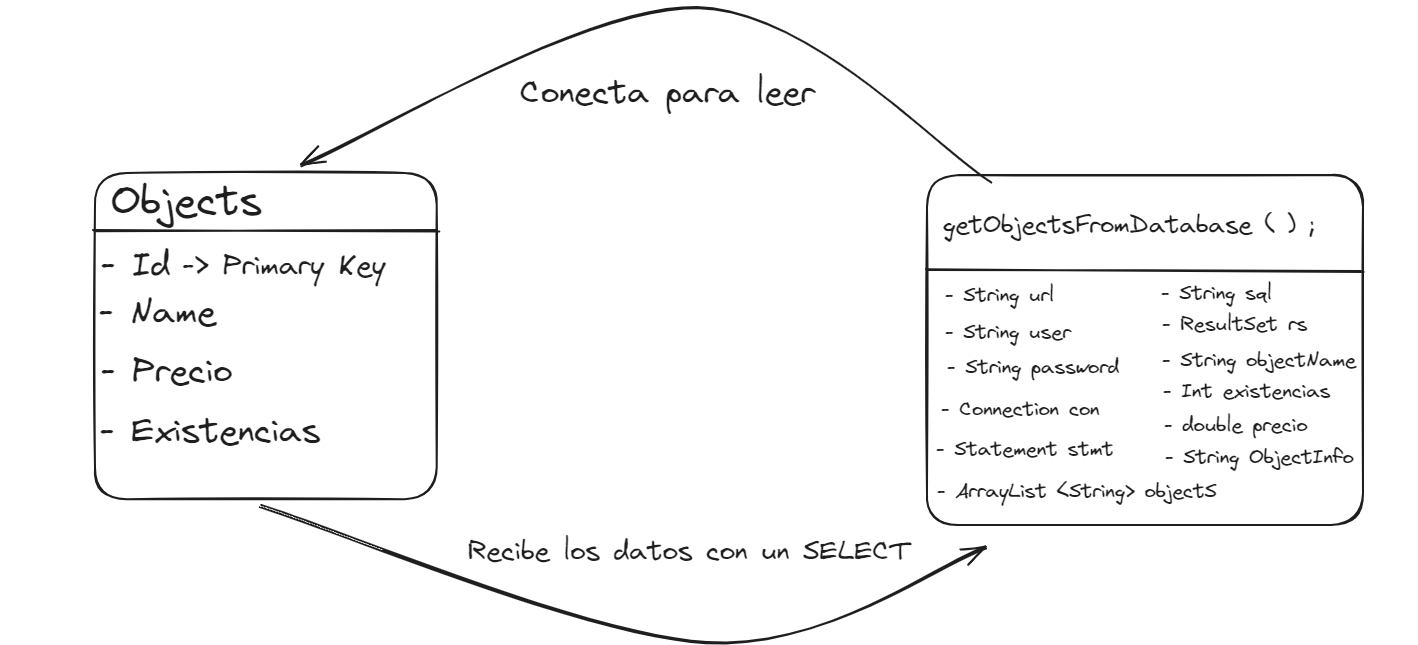
\includegraphics[width=0.7\textwidth]{Images/diagramabasededatoscomo.PNG}
    \caption{Imagen de como se leen los datos de la base de datos}
    \label{fig:diagramaBasededatosC}
\end{figure}
\clearpage
% ------------------------------------
Uno de los últimos métodos que merece la pena observar, es el método de checkear el volumen.
\begin{lstlisting}
    public void checkVol(){
    switch (volumeScale){
        case 0: volume = -80f; break;
        case 1: volume = -20f;break;
        case 2: volume = -12f;break;
        case 3: volume = -5f;break;
        case 4: volume = 1f;break;
        case 5: volume = 6f;break;
    }
    fc.setValue(volume);
}
\end{lstlisting}
Este método sigue la ecuación clásica de los decibelios:\\
\[
    \text{dB} = 20 \log_{10} \left( \frac{P}{P_0} \right)
\]

\text{Donde}:

\begin{itemize}
    \item \text{dB} \text{ es el nivel de sonido en decibelios}
    \item P \text{ es la presión acústica actual}
    \item P0 \text{ es la presión acústica de referencia}
\end{itemize}
Y este método se encargaría de realizar un checkeo al volumen, y ponerlo mediante un switch al volumen adecuado cambiando sus dBs.

\begin{flushright}
    \textit{Fórmula sacada del libro de Configuración de infraestructuras de sistemas de telecomunicaciones}
\end{flushright}
\clearpage
% ------------------------------------
\subsection{Base de datos}
Para la base de datos hemos optado por usar una sola tabla para listar los objectos que detallaremos a continuación, esta tabla contendría todos los datos de interés que necesitamos para el listado de objetos.\\
\begin{figure}[!ht]
    \centering
    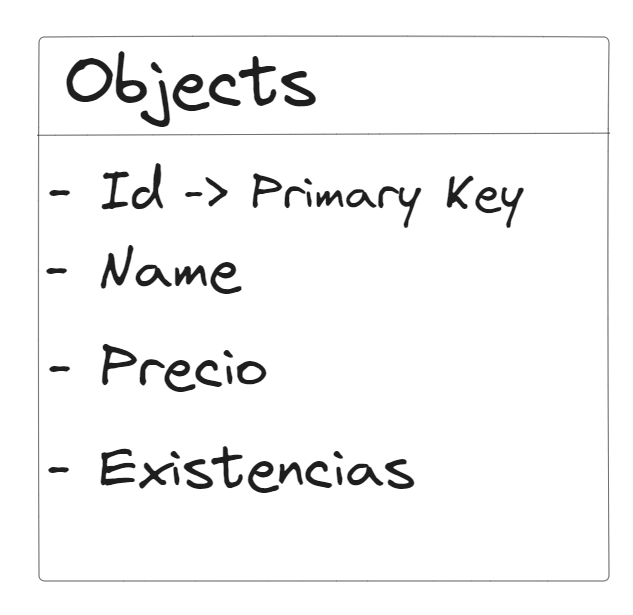
\includegraphics[width=0.3\textwidth]{Images/entidadRelacionBaseDeDatos.PNG}
    \caption{Imagen del diagrama de base de datos}
    \label{fig:diagramaBasededatos}
\end{figure}
Los atributos de la tabla son:
\begin{itemize}
    \item Id
          Necesario para poder buscar en concreto algún objeto en concreto dentro de la base de datos
    \item Name o Nombre
          Con este atributo ponemos un nombre medianamente descriptivo al objeto para que pueda ser reconocible por el jugador
    \item Precio
          Este atributo esta pensado para una versión futura del programa o propuesta de mejora, que sería el añadido del mercado, tener un precio en un juego donde existe el mercado, es importante ya que nos permite pensar si debemos vender o comprar el objeto.
    \item Existencias
          Otro dato pensado en una versión futura, ya que se podría realizar esta lista de forma interactiva con el juego, es decir al coger una existencia del listado de objetos, se podría eliminar una existencia del mismo.
\end{itemize}
Para poder realizar las dos últimas funcionalidades descritas en los atributos de la base de datos, habría que ampliar un poco más la base de datos y deberíamos quizás añadir algún atributo más. En el caso del precio,
no deberíamos añadir nada más ya que el mercader, leería directamente de la base de datos, lo único que necesitaríamos es que el jugador pueda realizar updates a la base de datos, ya que al comprar es lo que estaría haciendo, al vender no sería necesario, pues
por el momento no guardamos datos del jugador en la base de datos, en caso de tener una tabla que siga el progreso del jugador, si deberíamos realizar más operaciones en la base de datos.\\
Esto a futuro generaría un dilema, el cual es, qué usuario debería manipular la base de datos, ¿el usuario root?, No, para esto una idea que se me ocurre es crear otra tabla más, en este caso de usuarios y contraseñas, en esta tabla instaremos al usuario a registrarse según inicie el juego, mediante un sistema de login,
al realizar login, el usuario en su primera vez estaría creando en la base de datos un nuevo usuario, este nuevo usuario tendría permisos de update, select y delete, no necesita muchos más permisos, ya que solo queremos que lea de de la base de datos y manipule algún dato, darle más permisos podría provocar vulnerabilidades.
\clearpage
% ------------------------------------
\section{Fase de pruebas}
\subsection{Pruebas Unitarias}
\subsection{Entorno de pruebas}
\subsection{Rendimiento}
Para el rendimiento de la aplicación hemos usado un equipo con las siguientes características:
\begin{table}[htbp]
    \centering
    \caption{Especificaciones del equipo}
    \begin{tabular}{|l|l|}
        \hline
        \textbf{Componente} & \textbf{Detalle}                     \\
        \hline
        Placa base          & Gigabyte                             \\
        Procesador          & Intel Core i5 10600KF                \\
        GPU                 & NVIDIA GeForce RTX 3060 Ti OC VISION \\
        RAM                 & 32GB Kingston Fury                   \\
        Disco 1             & SSD 1TB M.2  NvME Kingston           \\
        Disco 2             & SSD 1TB 2.5 pulgadas                 \\
        Sistema Operativo   & Windows 11                           \\
        JDK                 & JDK 21                               \\
        \hline
    \end{tabular}
    \label{tab:equipo}
\end{table}
Las pruebas de rendimiento con este equipo no salieron favorables, es decir, mientras que el programa funcionaba perfectamente sin estar en pantalla completa, al ejecutar el programa en pantalla completa hemos determinado:\\
\begin{equation}
    \text{Porcentaje de caída de rendimiento} = \left( \frac{\text{FPS en ventana} - \text{FPS en pantalla completa}}{\text{FPS en ventana}} \right) \times 100
\end{equation}

\begin{equation}
    \left(\frac{60 - 50}{60}\right)\times 100 = \left( \frac{10}{60} \right) \times 100 = \frac{1}{6} \times 100 \approx 16.67 \%
\end{equation}

Como vemos el rendimiento cae un 16 \%, esto es algo a tener en cuenta y se puede estar produciendo por diferentes factores, el más obvio es que gráficamente no este utilizando el juego la tarjeta gráfica, ya que esta tarjeta es bastante potente para la tarea gráfica de este juego.
Aparte también creemos que puede estar relacionado con el buffer de swing, por lo que esto quizá se puede arreglar doblando el tamaño del buffer. Otra idea que puede ayudar al rendimiento, puede ser la de optimizar código. Dentro
de este proyecto contamos con cientos de líneas de código, las cuales, en su mayoría suponemos que pueden optimizarse.


\clearpage
% ------------------------------------
\section{Propuestas de mejora y trabajos futuros}
Dentro de esta sección vamos a nombrar ciertos apartados que se podrían añadir en una versión futura de la aplicación, y de paso, explicaremos alguna en detalle.\\
\textbf{Objetos rompibles}: empezamos con un clásico dentro de los videojuegos y son los objetos que se pueden romper, por ejemplo vasijas que oculten dinero, corazones, u otros objetos interesantes.\\
\textbf{Más personajes}: otro tema a tratar sería el número de personajes, se podría realizar algún tipo de selector de personajes o incluso una inclusión de un sistema de clases.\\
\textbf{Sistema de clases}: un clásico en los juegos de rol, sistemas de clases que en función, de cual elijamos, tendremos unas estadísticas u otra, y en un caso extremo, si escogemos un personaje mago podremos lanzar proyectiles mágicos y con un personaje como un caballero no.\\
\textbf{Jefes}: Aparte de algo obvio, como es extender más el juego, con nuevos mapas y enemigos, podemos llegar a poner Jefes, los cuales sean enemigos especiales, con ataques únicos y batallas incluso con puzzles.\\
\textbf{Misiones}: Un útlimo aspecto que podríamos meter, puede ser un sistema de misiones, en las cuales tengamos varios tipos de misiones, por ejemplo:
\begin{itemize}
    \item Misiones principales
          Misiones en las cuales se avanza en la historia principal del juego, necesarias para poder acabar el juego.
    \item Misiones secundarias
          Misiones en las que no se avanza en la historia principal, pero se hacen misiones bien más fáciles o bien más difíciles que las principales, que tengan una recompensa mayor o menor en función de la dificultad, esto nos permitiría añadir incluso mapas nuevos, enemigos opcionales y jefes opcionales incluso, así como armas secretas.
\end{itemize}
\textbf{Centralización de la base de datos}: Se detallará más abajo en un pequeño apartado, pero se podría centralizar la base de datos en un servidor central o ubicado por paises como el caso de los videojuegos actuales.
\textbf{Mercado}: Aunque se ha tratado de implementar una función de mercado o tradeo con un npc, no ha podido ser implementada sin errores a tiempo, por lo que queda como propuesta de mejora, ya que es una opción interesante, típica en videojuegos de este estilo, además serviría para que el jugador, pueda recuperar vida de otra manera.
\textbf{Guardado de partida}: Una función casi obligatoria en los videojuegos, guardar tu partida, ya sea en un archivo que genere el juego o en una base de datos, que guarde tu progreso.
\clearpage
% ---------------------------------
\subsection{Trabajos futuros}
En cuanto a trabajos futuros, cabe destacar la evolución de proyectos similares, que comenzaron como trabajos en escuelas, o universidades. Un ejemplo de esto, sería \textit{Stardew Valley}, es un videojuego que nació,
como TFG universitario, y su creador Eric Barone, también conocido como ConcernedApe, empezó desarrollándolo en su tiempo libre, y fue agregando funciones y refinando el juego hasta que se convirtió en un título muy interesante, sobre simulación de vida campesina,
con componentes RPG. \\
\textbf{Stardew Valley}\\
Es un simulador de vida rural en el que los jugadores deben gestionar una granja heredada del abuelo del personaje principal. A medida que los jugadores avanzan, pueden cultivar, criar animales, pescar, minar, y entablar relaciones con los NPCs (personajes no jugables) del pueblo. La calidad de estas relaciones influye en los objetos y recompensas que los NPCs ofrecen. Esta mezcla de simulación y elementos RPG ha capturado la atención de una gran audiencia, demostrando que un proyecto nacido de un TFG puede evolucionar significativamente con dedicación y tiempo.\\
Algunos conceptos clave de este juego son:
\begin{itemize}
    \item Simulación de granjas
    \item Componentes RPG
    \item Evolución del proyecto, empezó como proyecto académico
\end{itemize}
Otro ejemplo que nos puede venir a la cabeza, es \textit{Forager}, un videojuego de tipo farming y exploración, desarrollado por \textit{HopFrog}. En este juego, los jugadores,
deben producir recursos de la manera más eficiente, lo que parece simple al principio, pero en fases avanzadas se complica. La meta es construir una mejor base y explorar diversas islas, que cuentan con puzzles.\\
Algunos conceptos clave de forager son:
\begin{itemize}
    \item Gestión de recursos
    \item Exploración y Puzzles
    \item Progresión de dificultad
\end{itemize}
Estos ejemplos se pueden aplicar a Eldoria ya que, nos proveen de conceptos como:
\begin{itemize}
    \item Mejora continua
    \item Expansión de funcionalidades
    \item Optimización de la experiencia de juego
\end{itemize}
\begin{figure}[ht]
    \centering
    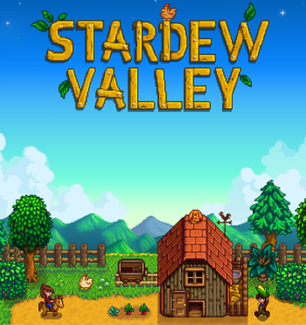
\includegraphics[width=0.3\textwidth]{Images/Logo_of_Stardew_Valley.png}
    \caption{Imagen de Stardew Valley}
    \label{fig:stardewValley}
\end{figure}
\clearpage
% ------------------------------------
\subsection{Bases de datos en otros videojuegos}
Otro concepto que también podríamos tener en cuenta es la tienda o mercado, es decir, hay muchos videojuegos actualmente que cuentan con una base de datos, por ejemplo, el videojuego \textit{Black Desert Online}, cuenta con un sistema de mercado, por medio de base de datos NoSQL, que es bastante extenso.
Cabe destacar que este videojuego, gestiona miles de jugadores por segundo, ya que se trata de un videojuego de rol de multijugador masivo, es por eso, que necesita una base de datos muy rápida, estamos hablando de que existen millones de objetos en este videojuego con los que se gestionan operaciones mercantiles,
incluso, existen miles de existencias de un mismo objeto que se vendan a diferentes precios, no es raro, encontrar un objeto vendiéndose a 30 mil monedas de juego y a 32 mil monedas de juego a la vez por diferentes personas, si a eso le sumamos, que cada persona puede poner las existencias que posea y quiera, estamos hablando,
de que diariamente se estarían produciendo, millones de operaciones mercantiles sobre la base de datos, en un videojuego que acoge de media 200 mil jugadores aproximadamente. Como vemos, las cifras son gigantes, pero encontramos un patrón, juegos de este estilo, como el \textit{World of Warcraft}, \textit{Dota 2} o \textit{Final Fantasy XIV}, tienen en común,
que usan bases de datos NoSQL, mientras que juegos menos pesados y con menos volumen de jugadores o de operaciones en la base de datos, usan bases de datos SQL, es el ejemplo de \textit{Clash of Clans}, que se trata de un juego móvil con un gran número de jugadores pero que en su base de datos, solamente almacena el progreso de cada jugador.
Como vemos, en videojuegos con un alto número de operaciones, se usan bases de datos NoSQL, mientras que en juegos que requieren base de datos, pero no quieren usar por ejemplo bases de datos NoSQL, y usan SQL, vemos que suelen almacenar información del usuario y no del juego, como usuario, contraseña y alguna estadística del mismo dentro del juego.\\
Es por ello que \textbf{otra propuesta de mejora} sería centralizar la base de datos en un servidor, como hacen la mayoría de videojuegos, de esta manera podríamos alquilar un host en \textit{AWS} y a partir de ahi generar algun sistema de login dentro del juego que almacene el progreso del jugador y sus objetos, como por ejemplo hace \textit{Activision}, con sus juegos de \textit{Call of Duty}.
\begin{figure}[ht]
    \centering
    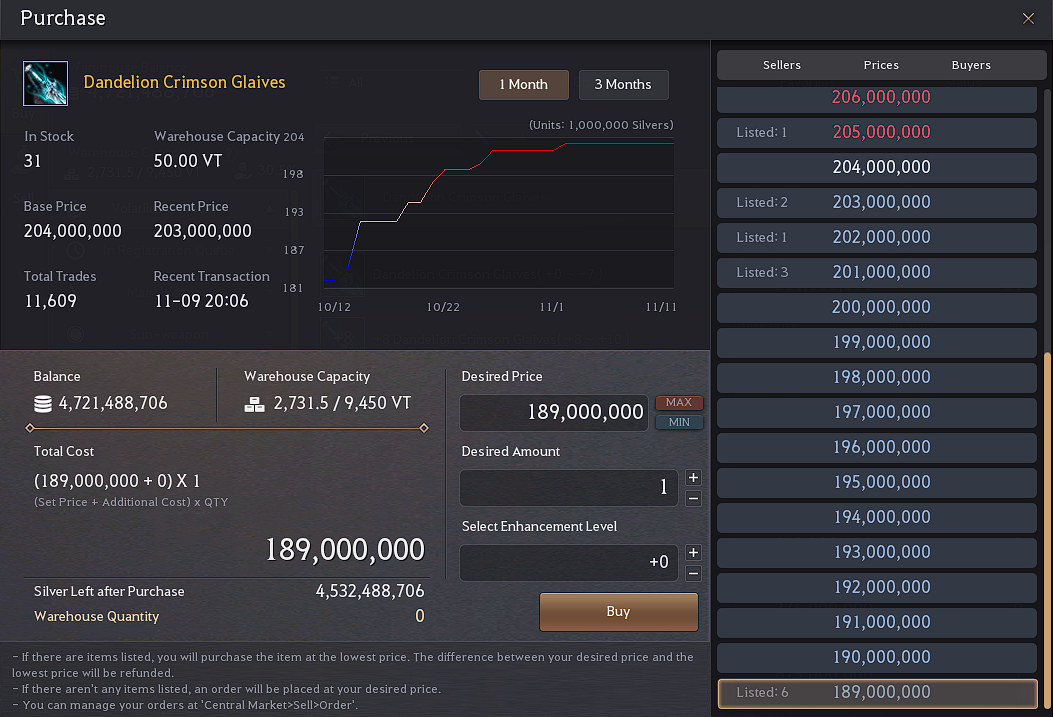
\includegraphics[width=0.8\textwidth]{Images/itemblackdesert.png}
    \caption{Imagen de Black Desert Online, item en venta}
    \label{fig:blackdesertfigure}
\end{figure}
\clearpage
% ------------------------------------
\section{Repositorios del Proyecto}
Este proyecto, se divide en dos repositorios, uno que contiene el código de la aplicación y otro que contiene la documentación del mismo, adjuntamos foto de ambos.
\begin{figure}[ht]
    \centering
    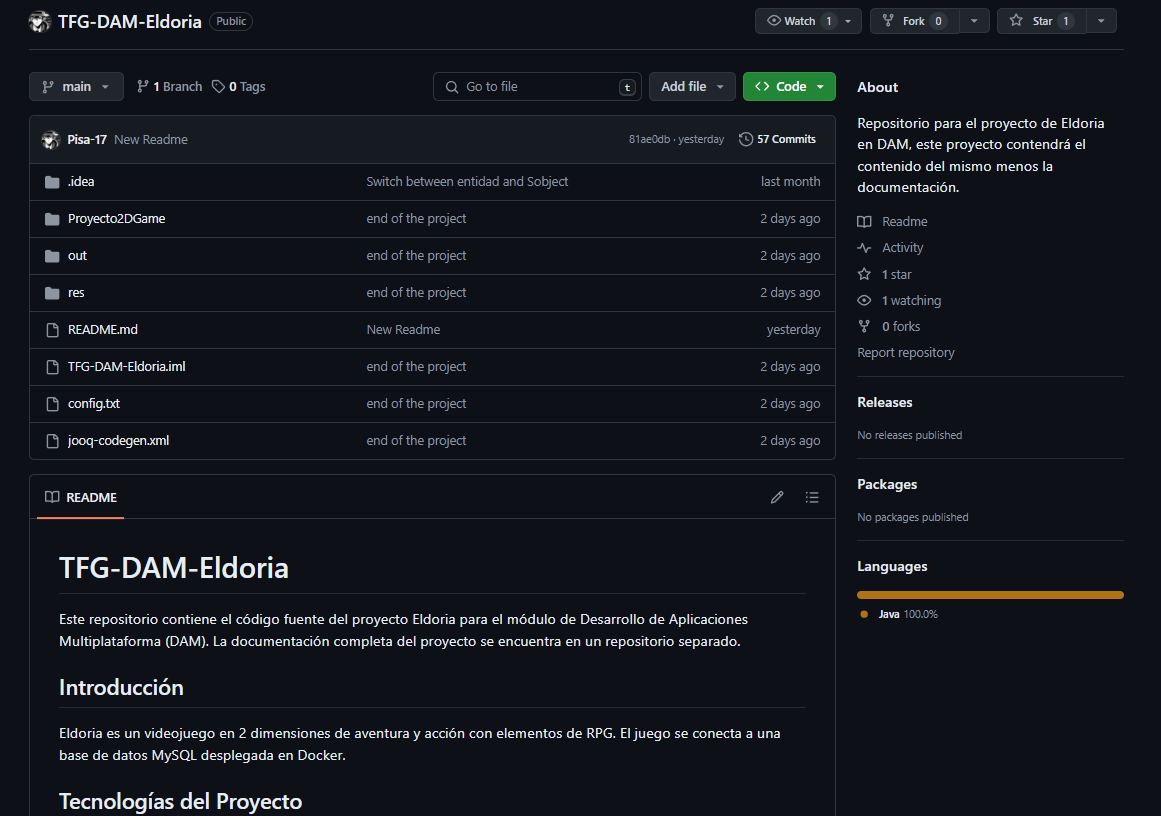
\includegraphics[width=0.6\textwidth]{Images/codigorepo.png}
    \caption{Repositorio del codigo}
    \label{fig:codigorepo}
\end{figure}
\begin{figure}[ht]
    \centering
    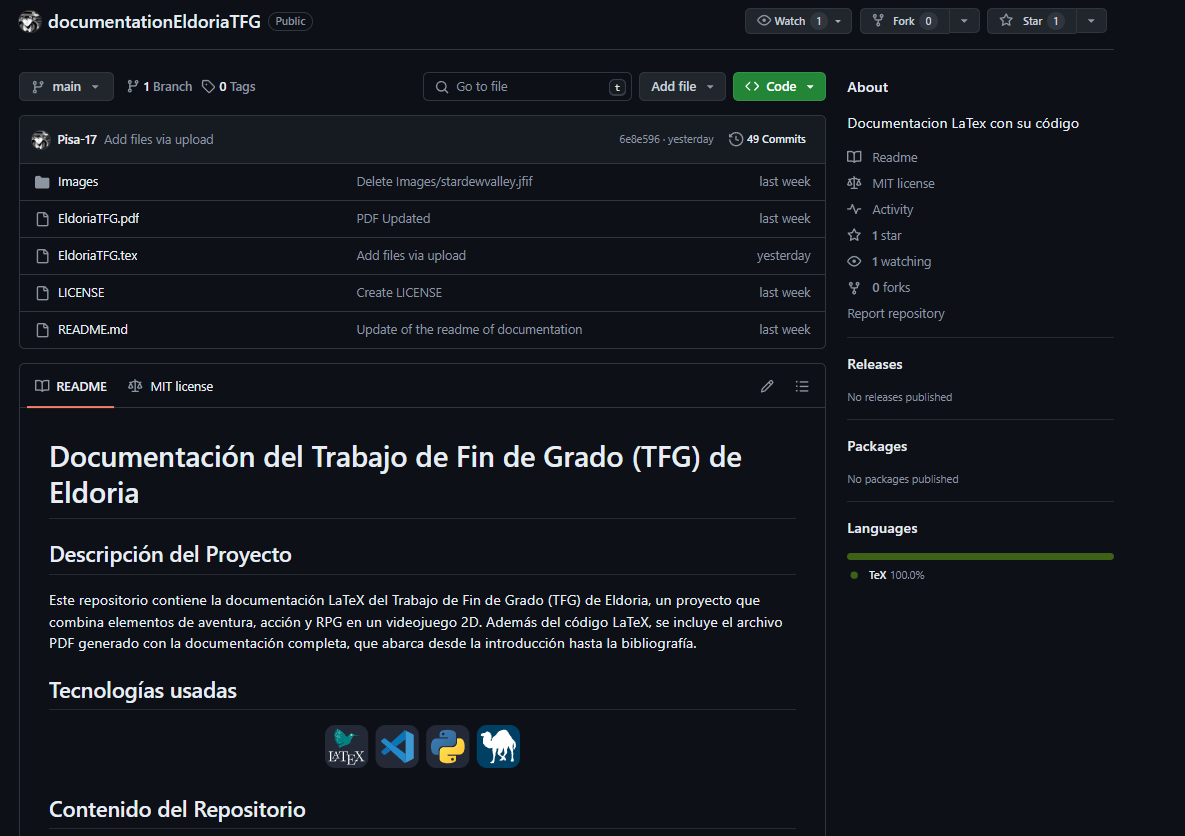
\includegraphics[width=0.6\textwidth]{Images/documentacionrepo.png}
    \caption{Repositorio de la documentación}
    \label{fig:documentacionrepo}
\end{figure}
\clearpage
% ------------------------------------
\subsection{Readme de los repositorios}
Vamos a enseñar brevemente el readme de ambos repositorios, cabe destacar que no es el readme entero y se recomienda ehcar un ojo a ambos repositorios
\begin{figure}[ht]
    \centering
    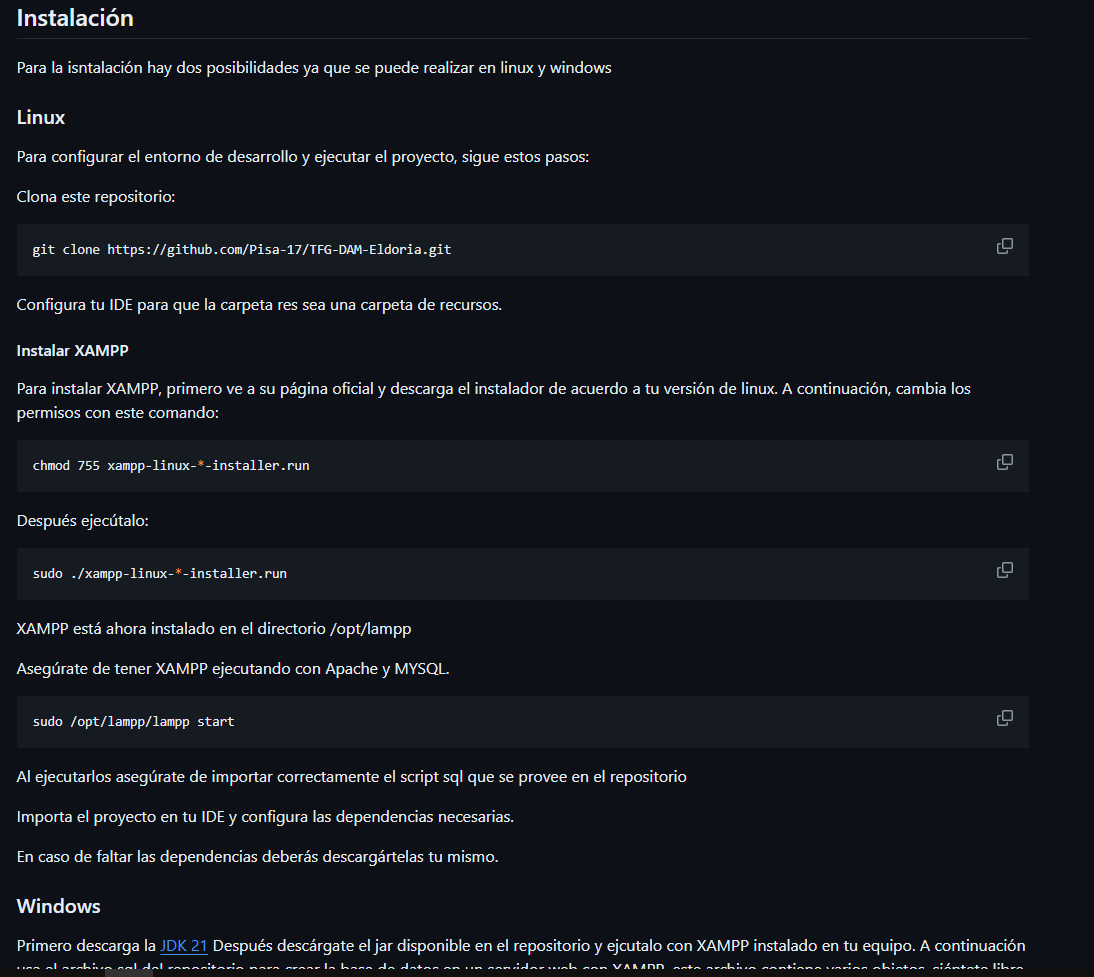
\includegraphics[width=0.6\textwidth]{Images/readmecodigorepo.png}
    \caption{Readme del código}
    \label{fig:repocodreadme}
\end{figure}
\begin{figure}[ht]
    \centering
    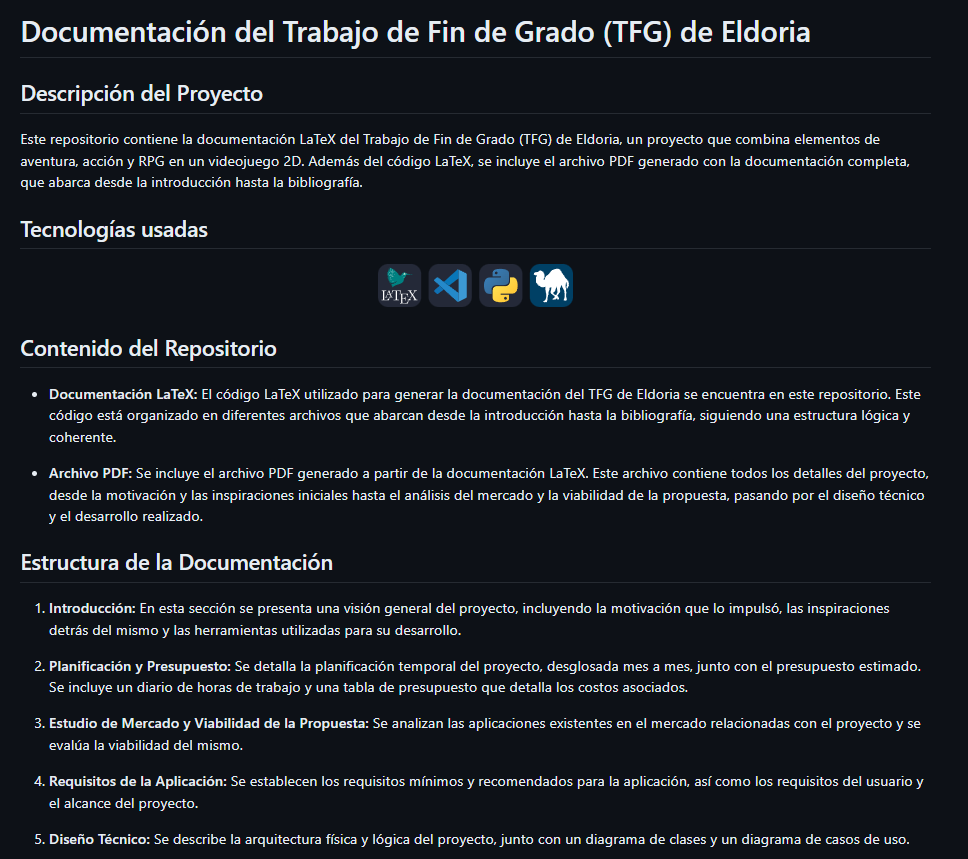
\includegraphics[width=0.5\textwidth]{Images/readmedocumentation.png}
    \caption{Readme de la documentación}
    \label{fig:documentacionreporeadme}
\end{figure}

\clearpage
% ------------------------------------
\section{Bibliografia}
% ------------------------------------
\begin{itemize}
    \item \textbf{\href{https://github.com/Pisa-17/TFG-DAM-Eldoria/tree/main}{Repositorio del juego}}
    \item \textbf{\href{https://github.com/Pisa-17/documentationEldoriaTFG/tree/main}{Repositorio de la documentación}}
    \item \textbf{\href{https://excalidraw.com/}{Excalidraw}}
    \item \textbf{\href{https://manualdelatex.com/}{Manual de LaTex}}
    \item \textbf{\href{https://mermaid.js.org/intro/getting-started.html}{Mermaid}}
    \item \textbf{\href{https://www.jetbrains.com/es-es/idea/}{IntelliJ}}
    \item \textbf{\href{https://www.piskelapp.com/}{Editor Pixel art}}
    \item \textbf{\href{https://tips.clip-studio.com/es-es/articles/2484}{Como hacer Assets}}
    \item \textbf{TFG de la Escuela de Segovia} - \url{https://uvadoc.uva.es/bitstream/handle/10324/24495/TFG-B%201042.pdf?sequence=1}
    \item \textbf{XAMPP} - \url{https://www.dongee.com/tutoriales/que-es-xampp/}
    \item \textbf{\href{https://stackoverflow.com/questions/1596009/java-lang-outofmemoryerror-java-heap-space}{Out Of Memory Error}}
    \item \textbf{Assets} - \url{https://pixel-boy.itch.io/ninja-adventure-asset-pack}
    \item \textbf{Autor de los Assets} - \url{https://twitter.com/2Pblog1}
    \item \textbf{JDBC} - \url{https://www.ibm.com/docs/es/informix-servers/12.10?topic=started-what-is-jdbc}
    \item \textbf{Visual Studio Code} - \url{https://code.visualstudio.com/Download}
    \item \textbf{Diagrama de clases IntelliJ} - \url{https://www.jetbrains.com/help/idea/class-diagram.html}
    \item \textbf{JDK 21} - \url{https://www.oracle.com/java/technologies/javase/jdk21-archive-downloads.html}
    \item \textbf{\href{https://medium.com/@dq_irfandi/the-nostalgia-effect-how-retro-games-influence-modern-gaming-8925be77694e}{Retro Art Article}}
    \item \textbf{\href{https://www.wired.com/story/why-retro-looking-games-get-so-much-love/}{Why retro games are so Loved?}}
    \item \textbf{How to list code in LaTeX} - \url{https://es.overleaf.com/learn/latex/Code_listing}
    \item \textbf{Libro - The Legend of Zelda Hyrule historia} - \url{https://en.wikipedia.org/wiki/The_Legend_of_Zelda:_Hyrule_Historia} - ISBN 978-1-61655-041-7
    \item \textbf{Web para hacer Diagramas de casos de uso online} - \url{https://online.visual-paradigm.com/drive/#infoart:proj=0&dashboard}
    \item \textbf{Landing on Blasphemous - Documental} - \url{https://youtu.be/lk--if_7J9g?si=kpGDZ2x66cMYwh1K}
    \item \textbf{Libro Configuración de infraestructuras de sistemas de telecomunicaciones} - ISBN 978-84-9732-934-7
    \item \textbf{Overleaf} - \url{https://es.overleaf.com/}
\end{itemize}

\clearpage
% ----------------------------------------

\begin{appendices}
    \renewcommand{\thesection}{} % Elimina la numeración de las secciones

    \section{Anexo I - Manual de Usuario}
    Los controles del juego son bastante simples, tendriamos las teclas \textit{W,A,S y D}, para mover el personaje y las teclas \textit{C, P, y ENTER} para otras acciones.
    \begin{itemize}
        \item W - Mover el personaje hacia arriba
        \item A - Mover el personaje a la izquierda
        \item D - Mover el personaje a la derecha
        \item S - Mover el personaje hacia abajo
        \item C - Ver las estadisticas del personaje
        \item P - Abrir el menu de Pausa y listado de objetos
        \item ENTER - Interactuar con NPCs, atacar, aceptar o continuar.
    \end{itemize}
    \clearpage
    % ---------------------------------------

    \section{Anexo II - Assets}
    Para las Assets del tfg hemos usado el siguiente paquete de assets: \\
    \url{https://pixel-boy.itch.io/ninja-adventure-asset-pack} \\
    Este paquete se puede descargar de forma gratuita ya que el autor nos deja pagar el precio que consideremos justo, el perfil del autor tambien lo podemos encontrar en la bibliografía. \\
    Vamos a ver que assets principales que hemos usado para este tfg en cuanto a este paquete se refiere:
    \begin{itemize}
        \item Ninja rojo - Personaje principal
              \begin{figure}[ht]
                  \centering
                  
\includegraphics[width=0.1\textwidth]{Images/FacesetPlayer.png}
                  \caption{Imagen del protagonista}
                  \label{fig:player}
              \end{figure}
              \begin{itemize}
                  \item Este sería el personaje principal de la avenutra, el \textit{Ninja rojo}, el cual sería en si el jugador también ya que es el personaje que controlamos con el teclado. Además este
                        personaje cuenta con un arma, la \textit{Katana}, la cual incialmente lleva equipada incialmente.
              \end{itemize}
        \item Cyclope - Enemigo
              \begin{figure}[ht]
                  \centering
                  
\includegraphics[width=0.1\textwidth]{Images/monster1.png}
                  \caption{Imagen del cíclope}
                  \label{fig:ciclope}
              \end{figure}
              \begin{itemize}
                  \item El enemigo principal del juego, es el enemigo contra el que generalmente lucharemos a lo largo de la aventura.
              \end{itemize}
        \item Arboles Sakura
              \begin{figure}[ht]
                  \centering
                  
\includegraphics[width=0.1\textwidth]{Images/arboles.png}
                  \caption{Imagen del árbol}
                  \label{fig:arbol}
              \end{figure}
              \begin{itemize}
                  \item Esta sería el asset para el árbol que adorna parte del mundo.
              \end{itemize}
              \clearpage
              % ------------------------------------
        \item Tiles - Casillas
              \begin{figure}[ht]
                  \centering
                  
\includegraphics[width=0.1\textwidth]{Images/cesped1.png}
                  \caption{Imagen del césped}
                  \label{fig:cesped}
              \end{figure}
              \begin{itemize}
                  \item Este sería el césped usado, uno de los varios assets del juego.
              \end{itemize}
              \begin{figure}[ht]
                  \centering
                  
\includegraphics[width=0.1\textwidth]{Images/agua.png}
                  \caption{Imagen del agua}
                  \label{fig:agua}
              \end{figure}
              \begin{itemize}
                  \item Asset usado para el agua del juego.
              \end{itemize}
              \begin{figure}[ht]
                  \centering
                  
\includegraphics[width=0.1\textwidth]{Images/arena.png}
                  \caption{Imagen de arena o camino}
                  \label{fig:arena}
              \end{figure}
              \begin{itemize}
                  \item Asset usado para simular un camino dentro del mapa.
              \end{itemize}
              \begin{figure}[!ht]
                  \centering
                  
\includegraphics[width=0.1\textwidth]{Images/rocas.png}
                  \caption{Imagen de las rocas}
                  \label{fig:rocas}
              \end{figure}
              \begin{itemize}
                  \item Asset usada para las rocas del mapa.
              \end{itemize}
              Y con esto acabarían los asset relativos a los tiles, es decir a las casillas del mapa, sobre el que se desarrollará el videojuego, cabe decir, que el 90\% de ellos vienen de un pack referenciado en la bibliografía.
              \clearpage
              % -----------------------------------
        \item Monje - NPC de la fase de pruebas
              \begin{figure}[!ht]
                  \centering
                  
\includegraphics[width=0.1\textwidth]{Images/monje.png}
                  \caption{Imagen del monje}
                  \label{fig:monje}
              \end{figure}
              \begin{itemize}
                  \item El famoso npc llamado \textit{sabio}, este npc fue el que hemos usado durante el desarollo para probar dialogos e interacciones con el jugador.
              \end{itemize}
        \item Katana - Arma inicial
              \begin{figure}[!ht]
                  \centering
                  
\includegraphics[width=0.05\textwidth]{Images/katana.png}
                  \caption{Imagen de la katana}
                  \label{fig:katana}
              \end{figure}
              \begin{itemize}
                  \item Arma principal del protagonista, con esta arma empieza el videojuego el protagonista.
              \end{itemize}
        \item Rapier - Arma avanzada
              \begin{figure}[!ht]
                  \centering
                  
\includegraphics[width=0.05\textwidth]{Images/rapier.png}
                  \caption{Imagen del estoque o rapier}
                  \label{fig:rapier}
              \end{figure}
              \begin{itemize}
                  \item Asset usado para el estoque o rapier, un arma más poderosa que la katana que inflinge algo más de daño.
              \end{itemize}
    \end{itemize}
    \clearpage
    % ---------------------------------------

    \section{Anexo III - Arte e inspiraciones detalladas}
    Dentro del apartado artistico debemos remontarnos a una época pasada, ya que tomamos muchos aspectos de juegos de décadas anteriores que nos han ayudado en cuanto a diseño, estética y cómo se ha
    diseñado el juego.

    \subsection{The legend of Zelda}
    Empezamos por la primera y clara inspiración que es \textit{The legend Of Zelda}, este videojuego bastante importante en la industria, sentó las bases para los próximos videojuegos de los siguientes años
    y es día de hoy que su fórmula sigue siendo un exito. La fórmula de este juego nos presenta una aventura de un héroe que debe rescatar a una princesa de un rey malvado, para ello durante la aventura se ganará
    el favor de las diosas de su mundo así como una espada sagrada para poder derrotar a este rey malvado. Esta fórmula gana mucho cuando nos metemos de lleno al juego, y dentro del juego lo que encontramos son puzzles,
    puzzles que nos proponen desafíos para superar las mazmorras y conseguir objetos. En los años 80 fue uno de los juegos más importantes. Mucha parte de la inspiración no llega solo por el diseño del juego, sino también
    incluso por atmosfera del juego, es decir, el TFG, contiene una atmosfera medieval de fantasía que casa muy bien con lo que esta saga tiene en general en la mayoría de sus videojuegos, ejemplos de esto serían:
    \begin{itemize}
        \item The legend of Zelda Minish cap
        \item The legend of Zelda
        \item The legen of Zelda Skyward Sword
    \end{itemize}

    \begin{figure}[ht]
        \centering
        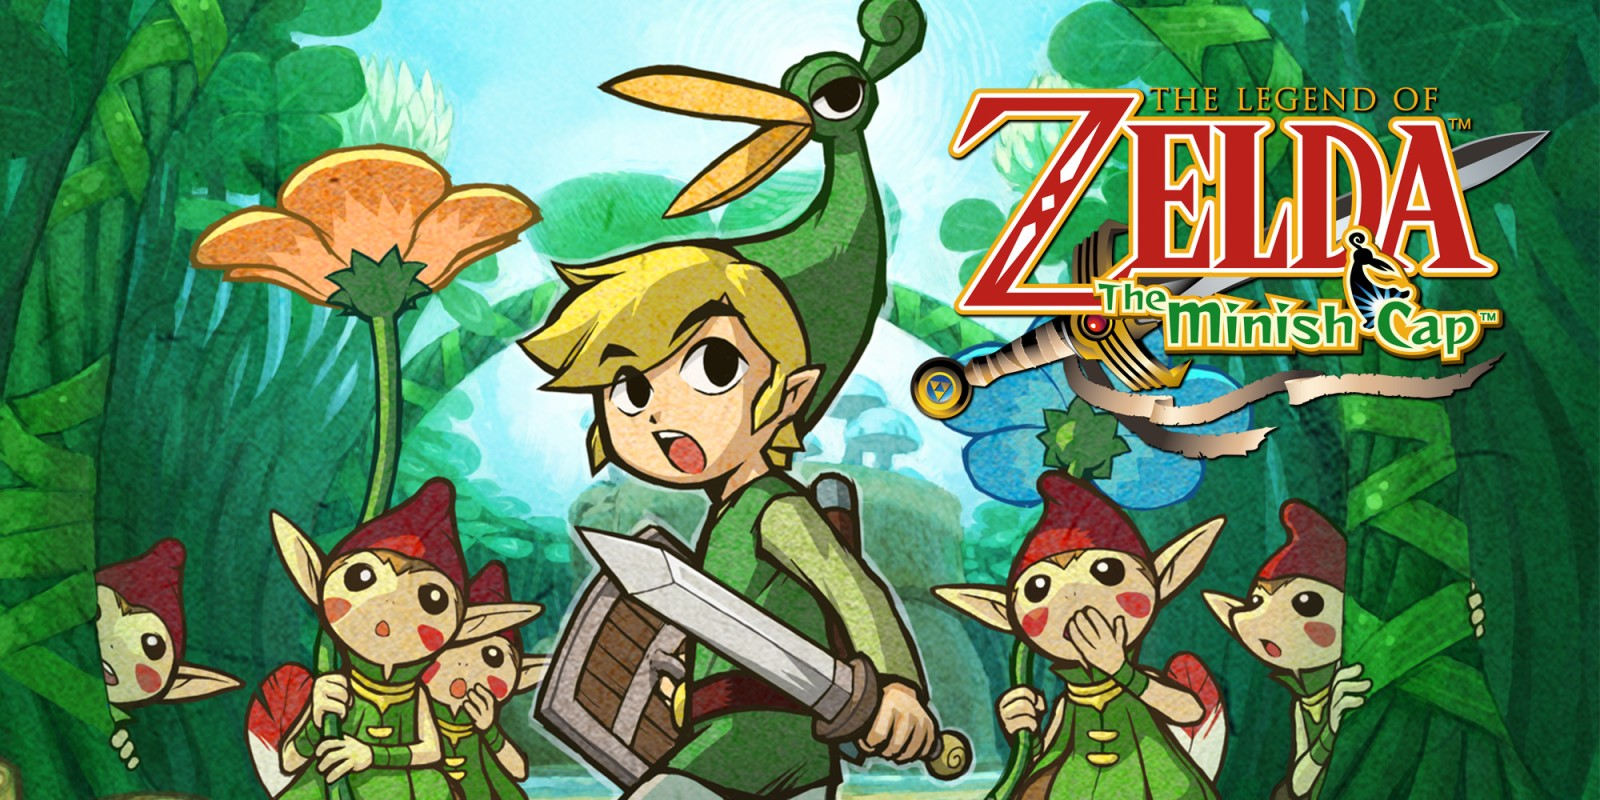
\includegraphics[width=0.6\textwidth]{Images/SI_GBA_TheLegendOfZeldaTheMinishCap_image1600w.jpg}
        \caption{The Legend Of Zelda Minish Cap}
        \label{fig:Zelda}
    \end{figure}

    Nótese también que esos videojuegos, salvo el último son videojuegos en 2 dimensiones que tienen una vista igual o similar a la presentada en Eldoria, es por ello que bebe mucho el TFG, de este tipo de fórmula que
    a dia de hoy, juegos grandes siguen usando, sin ir más lejos, \textit{The legend of Zelda Tears of the Kingdom}, sigue la fórmula del primero juego, varias mazmorras, en las que el jugador se enfrenta a varios puzzles,
    antes de llegar al jefe final del juego, debe pasar por varias pruebas e incluso optar a conseguir un arma legendaria para hacerle frente.

    \subsection{Final fantasy}
    La segunda inspiración tomada es otro juego de los años 80, el cual se llama \textit{Final Fantasy}, este juego se trata de un juego en dos dimensiones RPG por turnos que nos presenta una historia,
    acerca de 4 muchachos que se embarcan en la búsqueda de unos cristales mágicos que les servirán para disipar el mal de su mundo, durante la aventura se enfrentan a enemigos formidables y el juego tiene
    una estética de fantasía medieval. A dia de hoy esta saga sigue en desarollo, actualmente han sacado 16 juegos principales y varios secundarios.
    Pero, al igual que en el caso de la saga Zelda, encontramos la misma estructura que se repite en mayor o menor medida a lo largo de sus videojuegos, y de nuevo, en esta saga en lo que nos inspiramos es el ambiente,
    el ambiente medieval de fantasía tirando más a fantasia en este caso. Si bien es cierto que algún videojuego de esta saga, toca temas bastante profundos, nosotros en nuestro desarrollo hemos obviado realizar una historia
    relativamente compleja, ya que nos llevaría mucho más tiempo de lo normal. Un ejemplo de ello sería el \textit{Final Fantasy VII}, el cual es considerado uno de los mejores videojuegos de la historia, trata varios temas
    dificiles y complejos, y sigue teniendo la fórmula clásica tan característica de esta saga.

    \begin{figure}[ht]
        \centering
        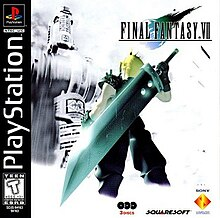
\includegraphics[width=0.6\textwidth]{Images/Final_Fantasy_VII_Box_Art.jpg}
        \caption{Final Fantasy VII}
        \label{fig:finalfantasy}
    \end{figure}

    \subsection{Blasphemous}
    La tercera inspiración ha sido un juego que se sale de los generos de RPG, se trata de un juego metroidvania, desarrollado en España, se trata de \textit{Blasphemous},
    un juego en dos dimensiones que nos pone en la piel del penitente, el cual entrará en un camino de penitencia y tendrá que realizar humillaciones para devolver el orden a su mundo, Cvstodia.
    Este juego presenta inspiración en mi proyecto ya que se trata de un juego con estética \textit{pixel art}, que es relativamente reciente. Este videojuego nos ha servido de inspiración ya que,
    al visualizar el documental acerca de como se ha desarrollado el juego, el cual hemos adjuntado en la bibliografía, podemos observar las complicaciones del mundo real, cuando queremos desarrollar un juego indie.
    Vemos como el tiempo siempre está ahí, como a veces, falta financiación, o como simplemente el equipo de desarrolladores se estresa mucho por las fechas limite.

    \begin{figure}[ht]
        \centering
        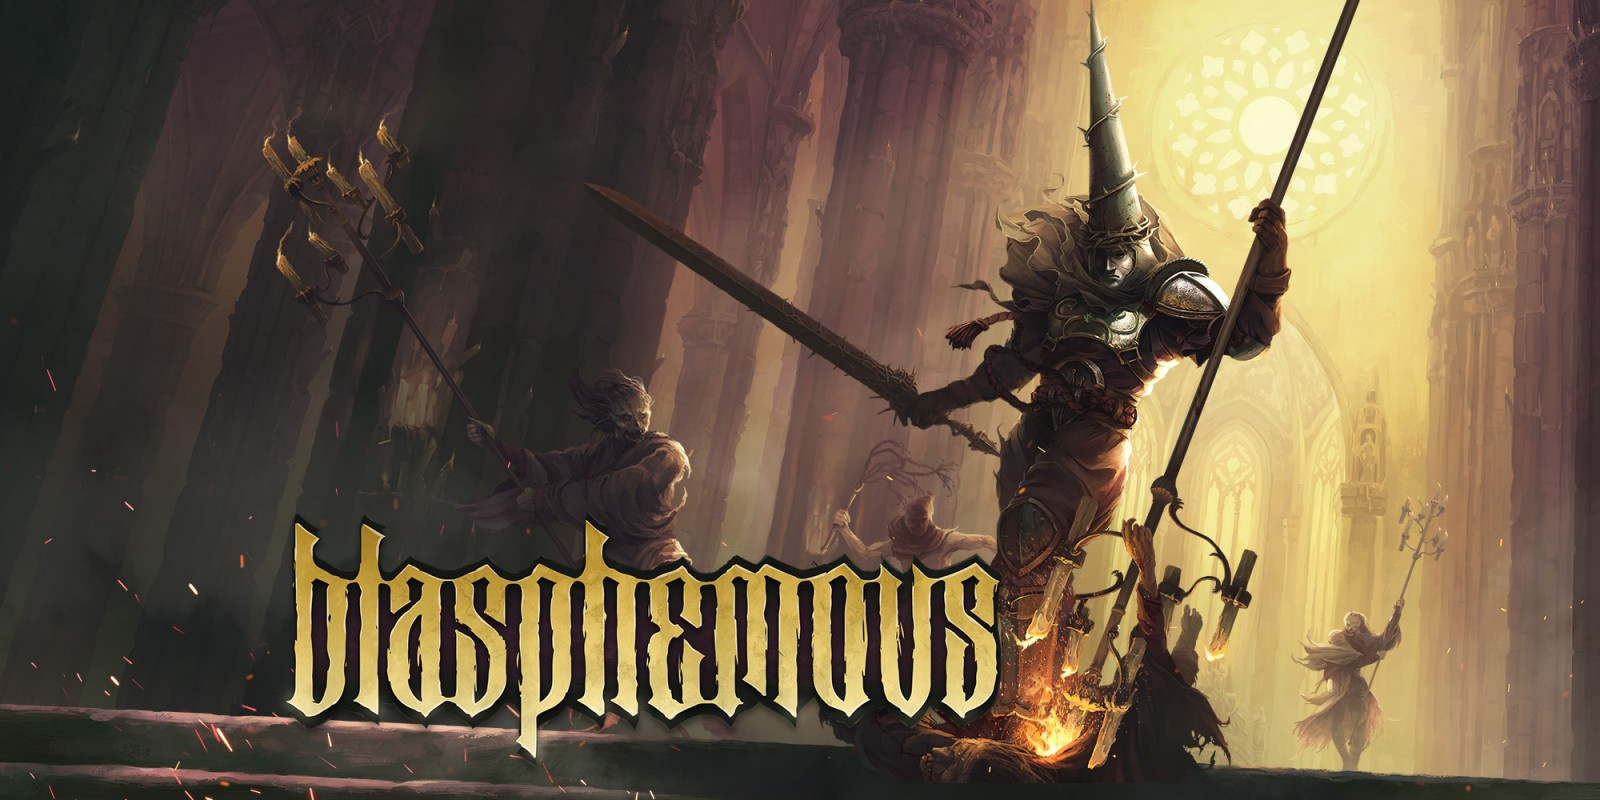
\includegraphics[width=0.6\textwidth]{Images/H2x1_NSwitchDS_Blasphemous_image1600w.jpg}
        \caption{Imagen de blasphemous}
        \label{fig:blasphemous}
    \end{figure}

    Es un documental que enseña, digamos, la cara oculta de desarrollar un videojuego, y esa cara oculta, son el estrés, la ansiedad, el no poder hacer quizás determinadas cosas por falta de tiempo, etc \dots
    Si bien es cierto que al final el producto que ha sacado este equipo de desarrolladores, ha sido una obra de una calidad muy alta, a mi me ha servido como mensaje de que se puede lograr lo que te propongas, con mucho esfuerzo,
    aparte de inspiración, ha sido una motivación que me ha llevado a realizar este TFG, además el videojuego al ser creado por un equipo Español, me ha animado mucho más.\\

    \begin{flushright}
        \textit{El equipo detrás del desarrollo de este videojuego fue The Game Kitchen}
    \end{flushright}
    \subsection{Arte del juego}
    El arte del juego sería una mezcla de todos los juegos ya mencionados excepto Blasphemous, ya que este último cuenta con sprites muy bien detallados y de mayor resolución.
    Se supone que el juego se desarrolla en una época medieval en la que existen magias, caballeros, dragones, ciclopes, etc \dots \\
    La mayoría de videojuegos de esta índole se desarrollan en épocas similares, remontandose en su mayoría al medievo europeo, o mundos mediavales con toques de fantasía que
    añaden juego a la hora de poder crear historias, personajes, escenarios, etc \dots \\
    Algunos ejemplos, aparte de los ya nombrados que siguen esta estética, podrían ser:

    \begin{itemize}
        \item Sea of stars
        \item Terraria
        \item Fire Emblem la saga completa
        \item V rising
    \end{itemize}

    \clearpage
    % ---------------------------------------

    \section{Anexo IV - Vocablos usados}
    Durante este documento se han hecho uso de varios vocablos de los que seguramente se desconozca el significado, tales como "FPS" por ejemplo, por ello vamos a recopilarlos aqui junto a su definicion.
    \begin{itemize}
        \item FPS Frames per second - Es la cantidad de imágenes que una pantalla puede mostrar en un segundo. Cuanto mayor sea el número de FPS, más suave y fluida será la visualización de un video o juego.
        \item RPG Role playing game - Es un género de videojuegos donde los jugadores asumen los roles de personajes en un mundo ficticio, siguiendo una narrativa y tomando decisiones que afectan la historia y el desarrollo del personaje.
        \item NPC Non Playable Character - Es cualquier personaje en un videojuego que no es controlado por el jugador, sino por la inteligencia artificial (IA) del juego. Estos personajes interactúan con el jugador, proporcionan información, misiones, desafíos, o ayudan a desarrollar la historia del juego.
        \item Inputs - Se refiere a las entradas del usuario al programa
        \item Pixel art - Estética basada en dibujar con pixeles solamente sin ningun arco o elemento circular
        \item Retro - Se refiere a una estética antigua, por ejemplo la de los juegos de los años 80
        \item Sprites - Son un conjunto de imágenes que representan un objeto o personaje
        \item Aspect ratio - La relación de aspecto es la proporción entre el ancho y la altura de una imagen, pantalla o cuadro visual. Se expresa como una relación matemática, por ejemplo, 16:9 o 4:3, donde el primer número representa el ancho y el segundo número la altura.
        \item Farming - En videojuegos se refiere a la práctica de repetir ciertas acciones o actividades en el juego con el objetivo de obtener recursos, experiencia, ítems, dinero del juego, o cualquier otro tipo de recompensa. Esta actividad es común en muchos géneros de videojuegos, especialmente en juegos de rol (RPG), juegos de estrategia, y juegos multijugador en línea masivos (MMO)
    \end{itemize}
    \clearpage
    % ---------------------------------------

\end{appendices}

\end{document}